\documentclass[runningheads]{llncs}
\usepackage{graphicx,amssymb,pepa,pgfplots,pgfplotstable,amsmath,placeins,listings}
\usetikzlibrary{patterns}

\begin{document}
\title{Performance modelling and simulation of skewed demand in complex systems}

\author{Stephen Shephard}

\institute{School of Computing Science, Newcastle University, Newcastle upon Tyne, NE1 7RU\\
	\email{s.shephard2@newcastle.ac.uk}}

\maketitle

%
% ---- Abstract and keywords
%
\begin{abstract}
On-line Transaction Processing (OLTP) applications must frequently deal with the issue of skewed demand for some resources.  This demand may overwhelm the whole system, affecting the owner's reputation and revenue.  This paper presents system architectures for a ticketing use case using a selection of distributed computing technologies of the Cloud.  It proposes models of these architectures and uses them to predict throughput in skewed demand scenarios.  The experimental results of the models are then tested against simple built systems.  It finds that the models correctly predict that a shared queue constrains throughput in proportion to relative demand, but overestimate the gains from a distributed database with replication.
	\keywords{Cloud, middleware, microservices, distributed databases, modelling, performance}
\end{abstract}

%
% ---- Introduction
%

\section{Introduction}\label{sec:introduction}

There are many high-profile examples of whole IT systems brought down by customer demand for part of their services.  Customers were prevented from using any part of the London 2012 Olympic ticketing website on launch day to avoid demand overloading the system \cite{RN1067}.  Demand for the finale of `True Detective' \cite{RN1066} brought down HBO Go.  Apple's iTunes Store suffered outage on the launch day of the iPhone 7 (new iPhone registration is carried out via an iTunes function) \cite{RN1068}.

This paper claims that it is possible to design and build more resilient systems through effective use of Cloud technologies where higher than normal demand for one function or type of resource would not block access to the others.  Skewed demand may be isolated so that it only affects parts of a system, or shared equally between different components. (The system may also adapt to demand by elastic scaling of resources, but this will not be considered as part of this paper).  When combining a middleware solution with a distributed database, however, where is the system bottleneck? If there are levels of demand that cannot be met on a limited budget, and that therefore some components will no longer meet the required throughput, what is the impact on the remainder of the system?

\subsection{Aims and Objectives}

The aim is to demonstrate that PEPA (Performance Evaluation Process Algebra) \cite{RN1051} may be used to construct models that are good predictors of the behaviour of real systems under skewed demand scenarios, and provide insights into the effectiveness of Cloud technologies for handling skewed demand.  The objectives are to show that:
\begin{itemize}
	\item distributed databases and middleware queues may be modelled in PEPA.
	\item these PEPA component models may be used to test skewed demand.
	\item the component models may be composed into system models with interesting behaviour under test.
	\item built system architectures for the PEPA models show behaviours predicted by the models.
\end{itemize}

\subsection{Methodology}

Performance models will be developed using a bottom-up approach from components to system architectures.  These will be iteratively tuned following development and measurement of built systems.

The paper is organised as follows.  Section \ref{sec:background} presents a use case based on ticket booking for a multi-sport event.  Section \ref{sec:technologies} selects a set of distributed technologies, and section \ref{sec:modelling} discusses modelling in PEPA.  Simple component models are proposed and tested in section \ref{sec:pepa-component-models} and composed into more complex system models in section \ref{sec:pepa-system-models} that make end-to-end predictions.  The models will then be tested against actual systems in section \ref{sec:built-systems}, built using Java and the Java Spring framework \cite{RN1076}, Cassandra \cite{RN1075,RN1050} databases, and where appropriate Microsoft Azure Storage Queues \cite{RN1072}.  These systems will be instrumented with Coda Hale Metrics \cite{RN1079} and measured under different scenarios of skewed demand, using Apache JMeter test plans \cite{RN1074}.  Finally section \ref{sec:conclusions} evaluates the approach and makes suggestions for future work.

%
% ---- Background
%

\section{Background}\label{sec:background}

Consider a general OLTP application using a distributed architecture, as shown in Figure \ref{figure:oltpapplication}.  Users access the application with a web-based front end.  Resources are stored in one or more databases.  In between the web servers and database are worker applications that service user requests, connected to the web servers by some middleware.  There are strategies for coping with skewed demand at each layer of this architecture.

\begin{figure}
	\centering
	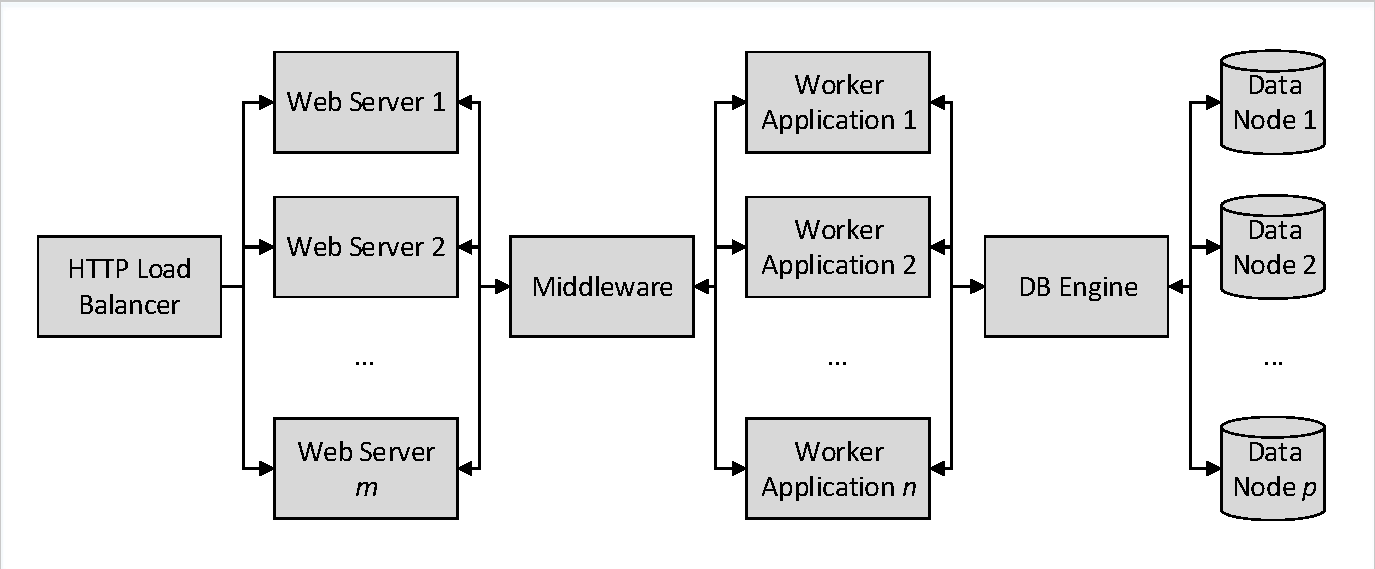
\includegraphics[trim = 5 5 5 5, clip, width=\textwidth]{img/application}
	\caption{OLTP application distributed architecture}
	\label{figure:oltpapplication}
\end{figure}

\paragraph{Adapting.} A system using {\itshape elastic scaling} may adapt to increased demand. Rapid elasticity is an essential characteristic of Cloud Computing by the NIST definition \cite{RN56}.  Computing resources, for example web servers or worker applications, can be elastically and often automatically scaled to meet current demand.  This gives the appearance of resources that are limited only by the system owner's budget.

\paragraph{Sharing.} High demand may be shared between resources.  HTTP load balancing improves the scalability of a web-based application by distributing the demand across multiple web servers \cite{RN73}.  Shared middleware such as a point-to-point queue, provides a competing consumer pattern to balance load from several producers, e.g. web servers, between multiple consumers e.g. worker applications.

\paragraph{Isolating.} If it is not possible to satisfy the skewed demand within a given budget, then it may be appropriate to isolate that demand from the rest of the system.  Horizontal partitioning of a distributed database can place high demand resources on different data nodes.  Microservices architecture offers a pattern for partitioning the data resources, the worker applications and the web servers, connecting them into entirely separate smaller end-to-end services.

\subsection{Use Case}

The concrete use case for constructing models and building systems is an application for searching, booking and returning tickets.  Following the Olympic example given in the Introduction, tickets will be for a multi-sport event.  Some sports are more popular than others and it will be assumed that there will be predictable skewed demand for {\itshape athletics} tickets.  Use cases where the resources with skewed demand are unknown - where they are only discovered once the application goes online, requiring some adaptive approach - are out of scope.  Such a ticketing application may be generalised to any system for allocating and releasing other resources with variable demand.

This paper considers the problem of higher than average demand for a particular type of ticket, and to what extent the system will allow users to search for other ticket types if some component is overloaded by the skewed demand for the most popular tickets.  It does not consider issues of fair allocation of scarce resources.

%
% ---- Technologies
%

\section{Technologies}\label{sec:technologies}

%
% ---- Choice of technologies in scope
%
\subsection{Scope}
\subsubsection{In Scope.}  The selected technologies in scope of this paper are shared middleware queues, distributed databases and microservices, which are discussed in more detail below.  The database partitioning strategy and entirely separate databases for the microservices architecture offer alternative means of isolating the skewed demand.  Using a single middleware queue shares and distributes the demand, this time in contrast to the microservices middleware approach.  The models will compare these approaches and investigate the behaviour of systems where the components have conflicting approaches to handling demand.
\subsubsection{Out of Scope.}  The paper will not consider elastic scaling or HTTP load balancing.  There is already a great deal of work in evaluating right-sizing strategies (minimising underutilisation and overutilisation of compute resources) for the former, e.g. \cite{RN49,RN62,RN48}.  HTTP load balancing is a relatively mature technology, and work has been done on simulation to evaluate different algorithms by response time and web server utilisation \cite{RN55}.

%
% ---- Queue Middleware
%

\subsection{Queue Middleware}\label{sec:middleware}

Good choice of middleware in a system will help ensure that its components are connected, but loosely coupled.  If, for example, a web server is blocked waiting for a response from a worker application carrying out a more expensive operation, then the throughput of the web server will be limited to that of the worker application.  The use case `return' operation however does not require a direct response from the system.  As long as the customer can rely on eventual guaranteed delivery of the return request, (and that the cost of their ticket will be refunded) then they do not need to wait for a direct response to their return.

Point-to-Point Queues, e.g. Azure Storage Queues \cite{RN1072}, are a form of Message-Oriented Middleware - an asynchronous, brokered message service providing an intermediate layer between senders and receivers, decoupling their communication.  Message delivery may take minutes rather than milliseconds, but the service providers do provide configurable delivery guarantees \cite{RN65}.  With synchronous middleware such as Remote Procedure Call (RPC), the calling process is blocked until the called service completes and returns control to the caller.  Distributed systems using asynchronous middleware do not block when calling a remote service.  Control is immediately passed back to the caller, and a response may be returned eventually, with the caller polling the remote service for the response, or the remote process calling a method in the caller to send the response.

Many processes may send messages to a queue, and each message is received by one consumer - though it may be one of several consumers competing for messages from this queue.  This competing consumer pattern offers a means of balancing load from the Web Servers between the Worker Applications in the ticketing use case.

%
% ---- Microservices
%
\FloatBarrier
\subsection{Microservices}\label{sec:microservices}

Microservices architecture is an approach to structuring applications as suites of small services, defined by business capability verticals rather than technological layers \cite{RN1069,RN1070}.  Each of the use case requirements - search for, book or return tickets - might typically be microservices with their own worker applications and data nodes.  Ticket data would be denormalised across the data nodes and made eventually consistent via a backplane messaging service \cite{RN1071} as shown in Figure \ref{figure:microservices}.  This would certainly isolate the demand for search, book and return from each other - returning tickets would not be blocked by a system where bookings were overloaded.  In the ticketing use case however, there is skewed demand for athletics tickets.  In a real-world system the booking microservice might be further broken down to a lower level of granularity to deal with this, i.e. a separate microservice for booking each ticket type.

\begin{figure}
	\centering
	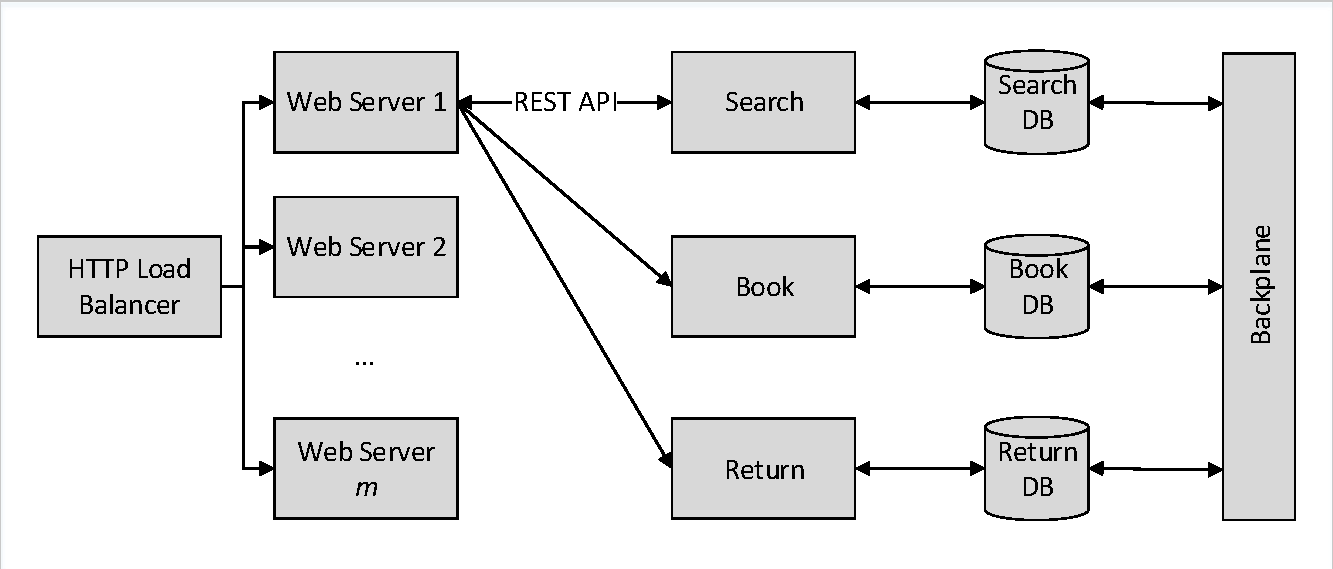
\includegraphics[trim = 5 5 5 5, clip, width=\textwidth]{img/microservices}
	\caption{Microservices}
	\label{figure:microservices}
\end{figure}

%
% ---- Distributed databases
%
\FloatBarrier
\subsection{Distributed databases}\label{sec:distributed-databases}
Modern SQL and NoSQL databases are designed to scale both data and the load of operations accessing that data over many servers that do not share disk or RAM, so-called `shared nothing' architecture \cite{RN67}.  We may partition data {\itshape vertically}, dividing tables into groups of columns that may be placed on different data nodes; or {\itshape horizontally}, where the split is by row \cite{RN68}. 

In the use case, the quantity of data does not approach the levels of `Big Data' applications.  Partitioning is proposed instead as a means of scaling the demand for that data.  The ticketing system will not require a large number of columns and the three operations outlined do not have significantly different column requirements, therefore horizontal partitioning is most relevant.  The partition key of a Ticket table may be the Ticket Type, the Date, or the seat Row.  Demand for tickets is likely to vary by each of these attributes.  An alternative partitioning strategy might be on the query, book and return operations.  The load on each data node would follow the demand for the data types and operations placed there.

One issue to be aware of is {\itshape replication}.   Most distributed databases offer replication of data from one partition to another for availability.  In the use case, if demand overloads a data node, the database may share the throughput using a copy of the data on another data node.  If this is also the primary data node of an otherwise low demand data type, then it may be overwhelmed in turn i.e. the skewed demand has followed the data.

\begin{figure}
	\centering
	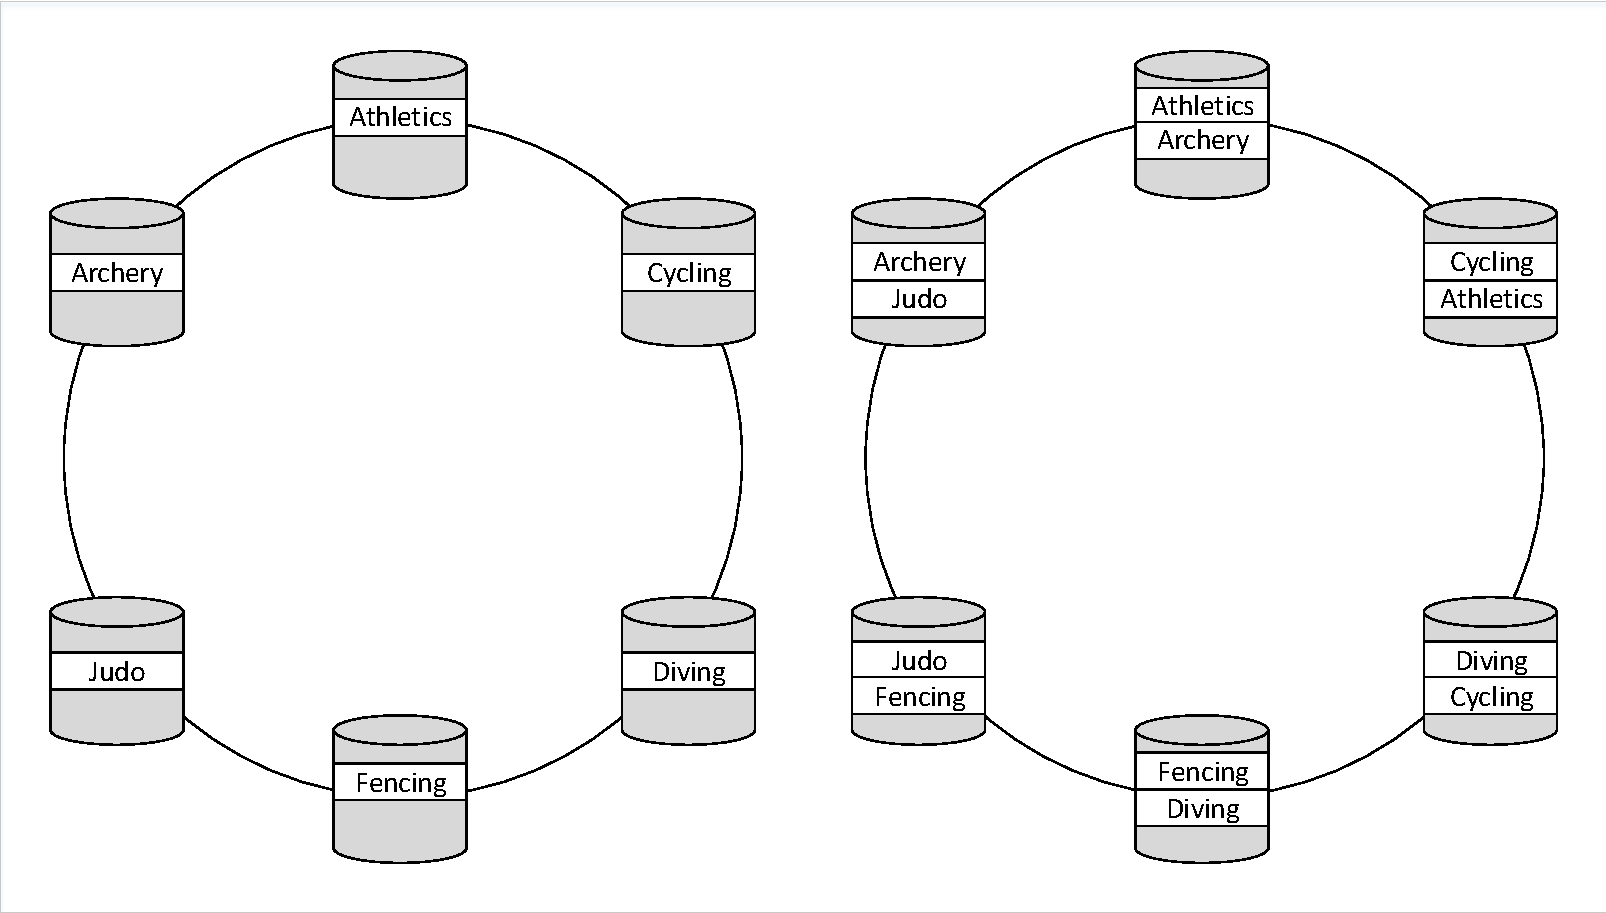
\includegraphics[trim = 5 5 5 5, clip, width=\textwidth]{img/dbdist}
	\caption{Consistent hashing, without and with replication}
	\label{figure:consistent_hashing}
\end{figure}
\FloatBarrier
The Cassandra database has an interesting method of partitioning data, using {\itshape consistent hashing} (also used by Riak, Redis and BigData among others \cite{RN66}).  The largest output of a hash function wraps round to the smallest value so that the range of hash values forms a conceptual `ring'.  Each data node is assigned a position on this ring, then the hash value of the partition key of a data item is used to determine the node used to store it.  When using replication, with a replication factor of {\itshape N}, a copy of the data is placed on the next {\itshape N-1} nodes walking clockwise round the ring \cite{RN1050}.  This is illustrated in Figure \ref{figure:consistent_hashing}.

\section{Modelling}\label{sec:modelling}

The modelling technique must enable predictions about throughput for varying levels of skewed demand.  It must also be possible to compose system models from simpler components.  Two current approaches for modelling cloud computing infrastructures are simulators or mathematical language-based models (e.g. {\itshape Process Algebra}).

\paragraph{Simulation Frameworks.} Several cloud simulation tools have been developed in recent years \cite{RN1081}, enabling the construction of models of Infrastructure as a Service environments.  They are often concerned with modelling the efficient running of that infrastructure, for example power usage, but also include utilisation models and may be useful for predicting the effect of shared demand or resource scheduling algorithms.  CloudSim \cite{RN69} is one such framework, requiring Java development for building the models.  This is an overhead for creation but offers flexibility in use.

\paragraph{Process Algebra.} Process Algebras (such as PEPA or TIPP \cite{RN64}) model throughput in interdependent processes, with a mixture of independent and shared actions operating at different rates.  There is a PEPA Eclipse plugin \cite{RN1080} that allows PEPA specifications to be parsed and run like programs, aiding experimentation on a range of action rates by automating repetitive calculations.

\subsection{PEPA (Performance Evaluation Process Algebra)}

The models will be produced using PEPA.  This paper is concerned with distribution of throughput in complex systems, rather than right-sizing those systems.  The Eclipse plugin will facilitate testing with a range of skewed demand values.

A PEPA model describes a system of interacting {\itshape components} which carry out {\itshape activities} at specified or passive {\itshape rates}.  A component is usually denoted by a name with an initial upper case letter, e.g. {\itshape Website}, and an activity type and rate are expressed as a bracketed pair e.g. $\mathit(request, r)$ where the activity type is normally a full lower case name and the rate is a single letter or the top symbol $\top$, denoting an unspecified (passive) rate.  There is a set of combinators that describe how the components and activities interact.  This paper uses the following subset, for the full syntax see {\cite{RN1051}}:

\subsubsection{Prefix:} $(\mathit{\alpha},\mathit{r}).\mathit{P}$ - a component carries out activity $\mathit{\alpha}$ at rate $\mathit{r}$ and then behaves as component $\mathit{P}$.
\subsubsection{Constant:} $\mathit{A} \rmdef \mathit{P}$ - assign the behaviour of component $\mathit{P}$ to the constant $\mathit{A}$.  Used with prefix, this can be used to define a recurring process e.g. $\mathit{P} \rmdef (\mathit{\alpha},\mathit{r}).\mathit{P}$.
\subsubsection{Choice:} $\mathit{P} + \mathit{Q}$ - a component may behave {\itshape either} as component $\mathit{P}$ or $\mathit{Q}$, non-deterministically.  This represents a race condition between components.
\subsubsection{Cooperation:} $\mathit{P} \sync{L} \mathit{Q}$ - for shared activities in the set $\mathit{L}$, components $\mathit{P}$ and $\mathit{Q}$ may only proceed with the simultaneous execution of those activities at the rate of the slowest component, otherwise they behave independently.
\subsubsection{Parallel:} $\mathit{P} \parallel \mathit{Q}$ - shorthand for components that synchronize with no shared activities i.e. equivalent to $\mathit{P} \sync{\emptyset} \mathit{Q}$.
\subsubsection{Aggregation:} $\mathit{P}[N]$ - represents $\mathit{N}$ instances of component $\mathit{P}$, but does not distinguish which instance of $\mathit{P}$ changes.  So for example where some component has states $\mathit{P1}$ and $\mathit{P2}$, and $\mathit{(P1|P2)}$ does not equal $\mathit{(P2|P1)}$, this model has 4 states.  If it doesn't matter which component has changed, then the model has only 3 states and can be written as $\mathit{P}[2]$.

\paragraph{Solutions.} PEPA models are used to represent a system using a stochastic process, where the activity durations are random variables.  Where these are negative exponentially distributed, then this representation is a continuous time Markov process with a steady state solution over a period of time \cite{RN1051}.  This may be calculated using the PEPA Eclipse plugin.

%
% ---- PEPA Component Models
%

\section{PEPA Component Models}\label{sec:pepa-component-models}

The first stage is to create suitable PEPA models for the selected technology components from section \ref{sec:technologies}, simple enough to be composed into more complex system models but still able to demonstrate interesting behaviour.  These models are tested using the PEPA Eclipse plugin \cite{RN1080} to calculate the steady-state throughputs of each activity for a given range of input rates for the activity with skewed demand.  The results are analysed to verify that the component models behave as expected for the technologies, and to discover any additional insights.  Note that there is no microservices component model.  Microservices is an architecture and will be shown in the System Modelling section.

%
% ---- Shared middleware queue
%
\FloatBarrier
\subsection{Shared middleware queue}

Work has already been done on modelling queueing systems in PEPA \cite{RN75}.  A single queue with a limited buffer size of $\mathit{N}$ may be written as (service and arrival components not shown, for brevity):

\begin{displaymath}
\centering
\begin{array}{rcl}
\mathit{Queue_0} & \rmdef & (\mathit{arrival},\mathit{\top}).\mathit{Queue_1}\\
\mathit{Queue_j} & \rmdef & (\mathit{arrival},\mathit{\top}).\mathit{Queue_{j+1}} + (\mathit{service},\mathit{\top}).\mathit{Queue_{j-1}}, \mathit{1 \le j \le N-1}\\
\mathit{Queue_N} & \rmdef & (\mathit{service},\mathit{\top}).\mathit{Queue_{N-1}}\\
\end{array}
\end{displaymath}

Using aggregation, this may be more simply represented in an easily extensible form as $\mathit{Queue[N]}$.  The limitation of this representation however is that it makes no distinction between the states of individual queue position instances, only the numbers of instances in each state.  This means there is no ordering guarantee e.g. the First In First Out (FIFO).  Actual cloud service queues do not necessarily implement FIFO, for example Azure Storage Queues \cite{RN1072} do not guarantee it.

For the skewed demand use case, a queue must be able to support arrival actions at different rates, and must potentially be able to support service actions in different ways too.  Again \cite{RN75} suggests an approach for this model, with a queue synchronised with a linear combination of components with different characteristics.  Thus the PEPA model for a general shared queue is shown in Figure \ref{figure:pepa_queue_model}.

There are two arrival processes, one dealing with the arrival of cycling requests at a uniform, normal rate (here set to $\mathit{c=1.0}$) and one dealing with the athletics requests at skewed rates (starting at the same rate as cycling requests, and increasing in steps of 1.0 to 10.0).  The queue itself is an aggregation of $\mathit{N}$ components each of which has three states; an empty instance $\mathit{Q_0}$, `filled' with an athletics request $\mathit{Q_A}$, or filled with a cycling request $\mathit{Q_C}$.  Finally there are also two service processes, generalised here to $\mathit{Service_1}$ and $\mathit{Service_2}$ (in some of the system models, they will not necessarily be dedicated to serving athletics or cycling requests), both with the same maximum service rate of $\mathit{s=5}$.  The higher rates of skewed demand are therefore more than the service processes can handle.

\begin{figure}
	\centering
	% Automatically generated by PEPA2Latex
	% --begin
	\begin{displaymath}
	\begin{array}{rcl}
	\mathit{a} & = & 1.0-10.0\\
	\mathit{c} & = & 1.0\\
	\mathit{s1} & = & 5.0\\
	\mathit{s2} & = & 5.0\\
	[2.0ex]		\mathit{Arrival_A} & \rmdef & (\mathit{athletics},\mathit{a}).\mathit{Arrival_A}\\
	\mathit{Arrival_C} & \rmdef & (\mathit{cycling},\mathit{c}).\mathit{Arrival_C}\\
	\mathit{Service_1} & \rmdef & (\mathit{serve1},\mathit{s1}).\mathit{Service_1}\\
	\mathit{Service_2} & \rmdef & (\mathit{serve2},\mathit{s2}).\mathit{Service_2}\\
	[2.0ex]		\mathit{Q_0} & \rmdef & (\mathit{athletics},\top).\mathit{Q_A}+(\mathit{cycling},\top).\mathit{Q_C}\\
	\mathit{Q_A} & \rmdef & (\mathit{serve1},\top).\mathit{Q_0}\\
	\mathit{Q_C} & \rmdef & (\mathit{serve2},\top).\mathit{Q_0}\\
	[2.0ex]		\multicolumn{3}{l}{\mathit{Arrival_A}\sync{athletics}\mathit{Q_0}[N]\sync{serve1}\mathit{Service_1}\sync{cycling}\mathit{Arrival_C}\sync{serve2}\mathit{Service_2}}\\
	[2.0ex]	\end{array}
	\end{displaymath}
	% --end
	\caption{Shared queue PEPA model}
	\label{figure:pepa_queue_model}
\end{figure}

\FloatBarrier
The model is tested in the Eclipse plugin using a series of different queue lengths $\mathit{N}$ and for different rates of athletics demand $\mathit{a}$ from 1 to 10.  This provides the actual throughputs in steady state of each activity.  Figure \ref{figure:queue_athletics} shows the throughput of {\itshape athletics} for exponentially increasing queue lengths from 1 to 20.  Figure \ref{figure:queue_cycling} shows the same for {\itshape cycling}.  Table \ref{table:queue_results} shows the numerical results for a queue of length N=10.
The results demonstrate that:
\begin{itemize}
	\item the throughput of {\itshape athletics} is constrained by the maximum service rate of the process handling those requests.
	\item the throughput of {\itshape cycling} is constrained by the ratio between the input rates of athletics and cycling.  When the input rate of athletics requests is 10 times that of cycling requests, then the queue holds these requests in a 10:1 ratio.  As the actual {\itshape athletics} throughput may not exceed the service rate $\mathit{s=5}$, then the cycling throughput is throttled to 0.5.
	\item for larger queue sizes, the throughputs approach their maximum limits.  A real queue service has an effectively unlimited length, but in PEPA models the state space quickly becomes too large for the Eclipse plugin to handle.  It is a useful result, therefore, to find that for a maximum skewed demand of 10 times the normal demand, a queue length of 10 gives a practical and well performing model.
\end{itemize}

\begin{figure}
	\centering
	\begin{tikzpicture}
	\begin{axis}[
	title={Throughput of athletics against input rate a for different queue lengths N},
	width=0.7\textwidth,
	xlabel={Rate a},
	ylabel={Throughput athletics},
	xmin=0, xmax=10,
	ymin=0, ymax=5,
	legend pos=north west,
	ymajorgrids=true,
	grid style=dashed,
	cycle multiindex* list={
		mark list*
		\nextlist
		cyan,brown,green,blue,red
	}
	]
	
	\addplot table [x index={0}, y index={1}, col sep=comma]{data/queue/N1_arrive_1.csv};
	\addplot table [x index={0}, y index={1}, col sep=comma]{data/queue/N2_arrive_1.csv};
	\addplot table [x index={0}, y index={1}, col sep=comma]{data/queue/N5_arrive_1.csv};
	\addplot table [x index={0}, y index={1}, col sep=comma]{data/queue/N10_arrive_1.csv};
	\addplot table [x index={0}, y index={1}, col sep=comma]{data/queue/N20_arrive_1.csv};
	
	\legend{N = 1, N = 2, N = 5, N = 10, N = 20}
	
	\end{axis}
	\end{tikzpicture}
	\caption{Shared queue experimental results - athletics}
	\label{figure:queue_athletics}
\end{figure}

\begin{figure}
	\centering
	\begin{tikzpicture}
	\begin{axis}[
	title={Throughput of cycling against input rate a for different queue lengths N},
	width=0.7\textwidth,
	xlabel={Rate a},
	ylabel={Throughput cycling},
	xmin=0, xmax=10,
	ymin=0, ymax=1,
	legend pos=south west,
	ymajorgrids=true,
	grid style=dashed,
	cycle multiindex* list={
		mark list*
		\nextlist
		cyan,brown,green,blue,red
	}
	]
	
	\addplot table [x index={0}, y index={1}, col sep=comma]{data/queue/N1_arrive_2.csv};
	\addplot table [x index={0}, y index={1}, col sep=comma]{data/queue/N2_arrive_2.csv};
	\addplot table [x index={0}, y index={1}, col sep=comma]{data/queue/N5_arrive_2.csv};
	\addplot table [x index={0}, y index={1}, col sep=comma]{data/queue/N10_arrive_2.csv};
	\addplot table [x index={0}, y index={1}, col sep=comma]{data/queue/N20_arrive_2.csv};
	
	\legend{N = 1, N = 2, N = 5, N = 10, N = 20}
	
	\end{axis}
	\end{tikzpicture}
	\caption{Shared queue experimental results - cycling}
	\label{figure:queue_cycling}
\end{figure}

\begin{table}[h!]
	\centering
	\caption{Shared queue N=10 experimental results}
	\label{table:queue_results}
	\pgfplotstabletypeset[
	col sep=comma,
	string type,
	columns/a/.style={column name=a, column type={p{.1\textwidth}}},
	columns/athletics/.style={column name=athletics, column type={p{.1\textwidth}}},
	columns/cycling/.style={column name=cycling, column type={p{.1\textwidth}}},
	columns/ratio/.style={column name=ratio, column type={p{.1\textwidth}}},
	columns/serve1/.style={column name=serve1, column type={p{.1\textwidth}}},
	columns/serve2/.style={column name=serve2, column type={p{.1\textwidth}}},
	every head row/.style={before row=\hline Rate & \multicolumn{5}{c}{Throughput} \\,after row=\hline},
	every last row/.style={after row=\hline},
	]{data/queue/N10_results.csv}
\end{table}

%
% ---- Database models
%
\FloatBarrier
\subsection{Database models}
A very simple representation of a single database process is a component that receives a request for data (either read or write) at some rate based on demand, and serves it at a rate based on the database's performance:
\begin{center}
	$\mathit{DB} \rmdef (\mathit{request}, r).(\mathit{dbsrv}, db).\mathit{DB}$
\end{center}
This is a highly abstract representation.  It does not model features such as session management, parallelism, caching, locking or any notion that data manipulation statements vary in complexity and expense.  Nevertheless it is a useful building block for distributed databases, as shown below.

%
% ---- Distributed database without replication
%
\FloatBarrier
\subsubsection{Distributed database.} Figure \ref{figure:pepa_ddnr_model} shows a model of a distributed database, where the data has been partitioned by sport onto two different database nodes with identical performance.  The data request activities are {\itshape athletics} and {\itshape cycling}.  These may represent search, book or return operations on athletics or cycling tickets.  Users may search for either type of ticket from the website component, and the code or database engine will route the search to the correct data node.  Thus $\mathit{DB_1}$ here is able to service {\itshape athletics} requests, at a maximum rate of {\itshape db}, and $\mathit{DB_2}$ can service {\itshape cycling} requests at the same rate (the model assumes homogeneous database nodes to reduce the variables under consideration, although as there are separate database service processes it is extensible to heterogeneous systems).  Both nodes execute in parallel without cooperating on any activities.

\begin{figure}
	\centering
	% Automatically generated by PEPA2Latex
	% --begin
	\begin{displaymath}
	\begin{array}{rcl}
	\mathit{a} & = & 1.0-10.0\\
	\mathit{c} & = & 1.0\\
	\mathit{db} & = & 5.0\\
	[2.0ex]		\mathit{Website} & \rmdef & (\mathit{athletics},\mathit{a}).\mathit{Website}+(\mathit{cycling},\mathit{c}).\mathit{Website}\\
	\mathit{DB_1} & \rmdef & (\mathit{athletics},\top).\mathit{DBsrv_1}\\
	\mathit{DBsrv_1} & \rmdef & (\mathit{dbsrv1},\top).\mathit{DB_1}\\
	\mathit{DB_2} & \rmdef & (\mathit{cycling},\top).\mathit{DBsrv_2}\\
	\mathit{DBsrv_2} & \rmdef & (\mathit{dbsrv2},\top).\mathit{DB_2}\\
	\mathit{Service_1} & \rmdef & (\mathit{dbsrv1},\mathit{db}).\mathit{Service_1}\\
	\mathit{Service_2} & \rmdef & (\mathit{dbsrv2},\mathit{db}).\mathit{Service_2}\\
	[2.0ex]		\multicolumn{3}{l}{\mathit{Website}\sync{\substack{athletics\\cycling}}\mathit{DB_1}\parallel\mathit{DB_2}\sync{\substack{dbsrv1\\dbsrv2}}\mathit{Service_1}\parallel\mathit{Service_2}}\\
	[2.0ex]	\end{array}
	\end{displaymath}
	% --end
	\caption{Distributed database PEPA model}
	\label{figure:pepa_ddnr_model}
\end{figure}

\FloatBarrier
Experiments are carried out in the Eclipse plugin by fixing the input rate of {\itshape db} at 5.0, the rate {\itshape c} of cycling requests to 1.0 and by testing each input rate {\itshape a} of athletics requests from 1.0 to 10.0 in steps of 1.0, to simulate increasing levels of skewed demand for athletics tickets which becomes too high for a single database node to service.  Table \ref{table:ddnr_results} shows the numerical results, and Figure \ref{figure:ddnr_sport} shows the throughput of both {\itshape athletics} and {\itshape cycling} against the skewed input rate {\itshape a}.
The results show that:
\begin{itemize}
	\item the throughput of {\itshape athletics} is constrained by the maximum service rate of the database node handling those requests, and both athletics and cycling activities demonstrate loss of throughput.
	\item the throughput of {\itshape cycling} is independent of athletics.
	\item the database node throughput follows the throughput of each sport activity, i.e. the partitioning strategy routes all the demand onto the node handling that sport.
\end{itemize}

\begin{table}[h!]
	\centering
	\caption{Distributed database without replication experimental results}
	\label{table:ddnr_results}
	\pgfplotstabletypeset[
	col sep=comma,
	string type,
	columns/a/.style={column name=a, column type={p{.1\textwidth}}},
	columns/athletics/.style={column name=athletics, column type={p{.1\textwidth}}},
	columns/cycling/.style={column name=cycling, column type={p{.1\textwidth}}},
	columns/dbsrv1/.style={column name=dbsrv1, column type={p{.1\textwidth}}},
	columns/dbsrv2/.style={column name=dbsrv2, column type={p{.1\textwidth}}},
	every head row/.style={before row=\hline Rate & \multicolumn{4}{c}{Throughput} \\,after row=\hline},
	every last row/.style={after row=\hline},
	]{data/ddnr/results.csv}
\end{table}

\begin{figure}
	\centering
	\begin{tikzpicture}
	\begin{axis}[
	title={Throughput against input rate a},
	width=0.7\textwidth,
	xlabel={Rate a},
	ylabel={Throughput},
	xmin=0, xmax=10,
	ymin=0, ymax=5,
	legend pos=north west,
	ymajorgrids=true,
	grid style=dashed,
	cycle multiindex* list={
		mark list*
		\nextlist
		cyan,brown,green,blue,red
	}
	]
	
	\addplot table [x index={0}, y index={1}, col sep=comma]{data/ddnr/book_a.csv};
	\addplot table [x index={0}, y index={1}, col sep=comma]{data/ddnr/book_c.csv};
	
	\legend{athletics,cycling}
	
	\end{axis}
	\end{tikzpicture}
	\caption{Distributed database without replication - sport throughput}
	\label{figure:ddnr_sport}
\end{figure}

%
% ---- Distributed database with replication
%
\FloatBarrier
\subsubsection{Distributed database with replication.}  Constructing and meaningfully testing a model of a distributed database using consistent hashing with replication requires at least three types of sport tickets, so a {\itshape diving} activity is introduced.  The partitioning strategy is as the previous model, but now $\mathit{DB_1}$ is able to service {\itshape athletics} and {\itshape cycling} requests,  $\mathit{DB_2}$ handles {\itshape cycling} and {\itshape diving}, and $\mathit{DB_3}$ handles {\itshape athletics} and {\itshape diving} as shown in Figure \ref{figure:pepa_ddwr_model}.  This model makes a key assumption that each data node handles each supported sport with equal probability, and once again each node operates at an identical rate that is insufficient to meet the skewed demand.

\begin{figure}
	\centering
	% Automatically generated by PEPA2Latex
	% --begin
	\begin{displaymath}
	\begin{array}{rcl}
	\mathit{a} & = & 1.0-10.0\\
	\mathit{c} & = & 1.0\\
	\mathit{d} & = & 1.0\\
	\mathit{db} & = & 5.0\\
	[2.0ex]		\mathit{Website} & \rmdef & (\mathit{athletics},\mathit{a}).\mathit{Website}+(\mathit{cycling},\mathit{c}).\mathit{Website}+(\mathit{diving},\mathit{d}).\mathit{Website}\\
	\mathit{DB_1} & \rmdef & (\mathit{athletics},\top).\mathit{DBsrv_1}+(\mathit{cycling},\top).\mathit{DBsrv_1}\\
	\mathit{DBsrv_1} & \rmdef & (\mathit{dbsrv1},\top).\mathit{DB_1}\\
	\mathit{DB_2} & \rmdef & (\mathit{cycling},\top).\mathit{DBsrv_2}+(\mathit{diving},\top).\mathit{DBsrv_2}\\
	\mathit{DBsrv_2} & \rmdef & (\mathit{dbsrv2},\top).\mathit{DB_2}\\
	\mathit{DB_3} & \rmdef & (\mathit{diving},\top).\mathit{DBsrv_3}+(\mathit{athletics},\top).\mathit{DBsrv_3}\\
	\mathit{DBsrv_3} & \rmdef & (\mathit{dbsrv3},\top).\mathit{DB_3}\\
	\mathit{Service_1} & \rmdef & (\mathit{dbsrv1},\mathit{db}).\mathit{Service_1}\\
	\mathit{Service_2} & \rmdef & (\mathit{dbsrv2},\mathit{db}).\mathit{Service_2}\\
	\mathit{Service_3} & \rmdef & (\mathit{dbsrv3},\mathit{db}).\mathit{Service_3}\\
	[2.0ex]		\multicolumn{3}{l}{\mathit{Website}\sync{\substack{athletics\\cycling\\diving}}\mathit{DB_1}\parallel\mathit{DB_2}\parallel\mathit{DB_3}\sync{\substack{dbsrv1\\dbsrv2\\dbsrv3}}\mathit{Service_1}\parallel\mathit{Service_2}\parallel\mathit{Service_3}}\\
	[2.0ex]	\end{array}
	\end{displaymath}
	% --end
	\caption{Distributed database with replication PEPA model}
	\label{figure:pepa_ddwr_model}
\end{figure}

Experiments are carried out in the Eclipse plugin by fixing the input rate of {\itshape db} at 5.0, the rates {\itshape c} and {\itshape d} of cycling and diving requests to 1.0 and by testing each input rate {\itshape a} of athletics requests from 1.0 to 10.0 in steps of 1.0.  The numerical results in Table \ref{table:ddwr_results} show that the throughputs of cycling and diving are identical.   Figure \ref{figure:ddwr_sport} therefore shows only the throughput of {\itshape athletics} and {\itshape cycling} against the skewed input rate {\itshape a} (the plots of cycling and diving would be superimposed).  Figure \ref{figure:ddwr_database} shows the throughput of all three database nodes against the same range of inputs.
The results show that:
\begin{itemize}
	\item the throughput of {\itshape athletics} is higher than for the distributed database without replication.  The extra demand has been shared between both data nodes supporting athletics requests.
	\item the throughput of {\itshape cycling} and {\itshape diving} are no longer independent of athletics.  They no longer reside only on data nodes that are independent of athletics demand.
	\item the database node throughput of the two nodes supporting athletics requests is equal, and both are higher than the remaining data node that supports only cycling and diving.  The throughput of this node increases as athletics throughput increases however, suggesting the node is picking up an increasing proportion of the constant demand for cycling and diving tickets.
\end{itemize}

\FloatBarrier
\begin{table}[h!]
	\centering
	\caption{Distributed database with replication experimental results}
	\label{table:ddwr_results}
	\pgfplotstabletypeset[
	col sep=comma,
	string type,
	columns/a/.style={column name=a, column type={p{.1\textwidth}}},
	columns/athletics/.style={column name=athletics, column type={p{.1\textwidth}}},
	columns/cycling/.style={column name=cycling, column type={p{.1\textwidth}}},
	columns/diving/.style={column name=diving, column type={p{.1\textwidth}}},
	columns/dbsrv1/.style={column name=dbsrv1, column type={p{.1\textwidth}}},
	columns/dbsrv2/.style={column name=dbsrv2, column type={p{.1\textwidth}}},
	columns/dbsrv3/.style={column name=dbsrv3, column type={p{.1\textwidth}}},
	every head row/.style={before row=\hline Rate & \multicolumn{6}{c}{Throughput} \\,after row=\hline},
	every last row/.style={after row=\hline},
	]{data/ddwr/results.csv}
\end{table}

\begin{figure}
	\centering
	\begin{tikzpicture}
	\begin{axis}[
	title={Throughput against input rate a},
	xlabel={Rate a},
	ylabel={Throughput},
	xmin=0, xmax=10,
	ymin=0, ymax=6,
	legend pos=north west,
	ymajorgrids=true,
	grid style=dashed,
	cycle multiindex* list={
		mark list*
		\nextlist
		cyan,brown,green,blue,red
	}
	]
	
	\addplot table [x index={0}, y index={1}, col sep=comma]{data/ddwr/book_a.csv};
	\addplot table [x index={0}, y index={1}, col sep=comma]{data/ddwr/book_c.csv};
	
	\legend{athletics,cycling}
	
	\end{axis}
	\end{tikzpicture}
	\caption{Distributed database with replication - sport throughput}
	\label{figure:ddwr_sport}
\end{figure}

\begin{figure}
	\centering
	\begin{tikzpicture}
	\begin{axis}[
	title={Throughput against input rate a},
	width=0.7\textwidth,
	ybar=0pt,
	bar width=.015\textwidth,
	xlabel={Rate a},
	ylabel={Throughput},
	xtick=data,
	ymin=0, ymax=5,
	legend pos=north west,
	ymajorgrids=true,
	grid style=dashed,
	]
	
	\addplot [pattern=north east lines, pattern color=blue] table [x index={0}, y index={1}, col sep=comma]{data/ddwr/dbsrv_1.csv};
	\addplot [fill=green] table [x index={0}, y index={1}, col sep=comma]{data/ddwr/dbsrv_2.csv};
	\addplot [pattern=crosshatch, pattern color=brown] table [x index={0}, y index={1}, col sep=comma]{data/ddwr/dbsrv_3.csv};
	
	\legend{dbsrv1,dbsrv2,dbsrv3}
	
	\end{axis}
	\end{tikzpicture}
	\caption{Distributed database with replication - database throughput}
	\label{figure:ddwr_database}
\end{figure}

%
% ---- PEPA System Models
%
\FloatBarrier
\section{PEPA System Models}\label{sec:pepa-system-models}
The components are combined into models of full distributed architectures, that may be implemented and tested as working built systems.  There are three system models - a simplified microservices architecture, and two models composed of a shared queue and distributed database, with and without replication.

%
% ---- Simple microservices
%
\FloatBarrier
\subsection{Simple microservices}

The simple microservices model has separate end-to-end services for handling athletics and cycling ticket requests.  This is not a `natural' microservices implementation, which would be more likely to separate on operations e.g. searching, booking and returning tickets.  Choosing this design however makes the system directly comparable to the partitioning strategy used for the distributed database models.  It is not in itself functionally different to separating services by operations unless considering additional features to handle eventual data consistency (see Future Work).

The system has two separate databases, one for athletics tickets, one for cycling, and each has its own dedicated worker application (Figure \ref{figure:simplemicro_architecture}).  The PEPA model of this (Figure \ref{figure:simplemicro}) uses the same database process building blocks as the distributed database component models, but in this case they cooperate with the dedicated worker application processes $\mathit{Worker_A}$ and $\mathit{Worker_C}$.

As for the component models, there are two arrival processes, dealing with cycling requests at the rate $\mathit{c=1.0}$ and athletics requests at rates 1.0 to 10.0 in steps of 1.0.  Again each database may serve requests at a maximum rate of {\itshape db}.  Note that this rate has been changed to 6.5 so that it is proportional to the performance observed when testing the built system (the model has been tuned following measurement of the system).

The worker application processes have a maximum rate of $\mathit{w=100.0}$.  This value has been chosen to be much higher than the other parts of the system to minimise its impact on the system testing.  The assumption being made here is that the applications may be designed to cope with this much higher demand, perhaps using Elastic Scaling of servers, which is out of scope of this paper.

\begin{figure}
	\centering
	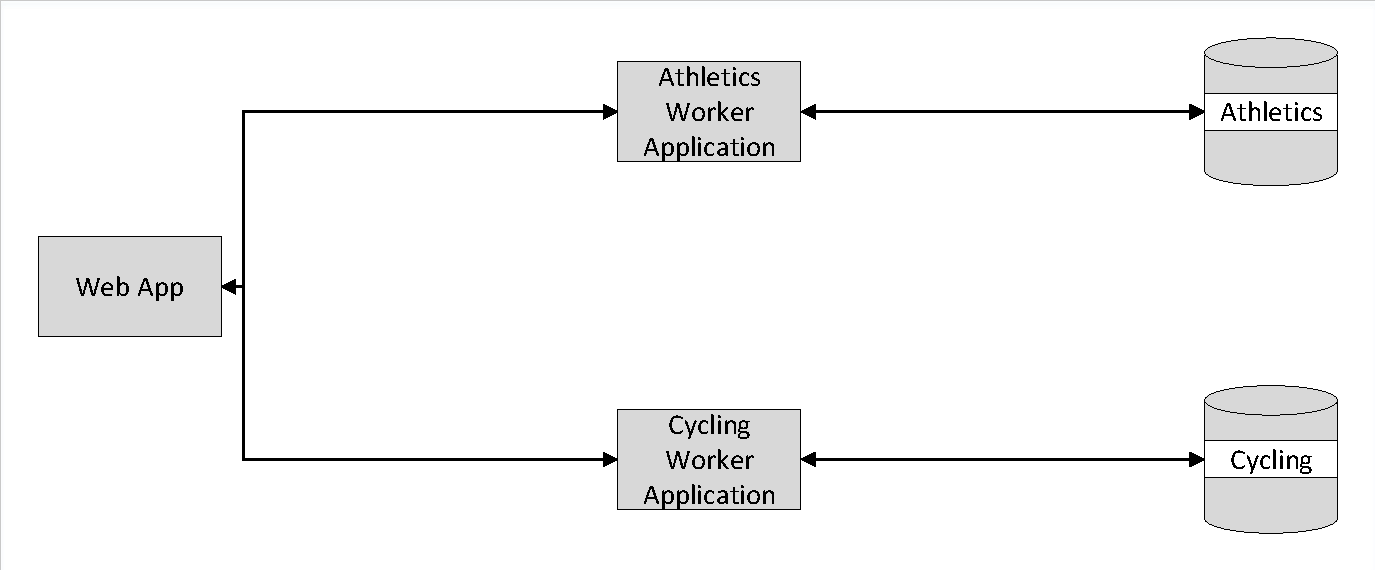
\includegraphics[trim = 5 5 5 5, clip, width=\textwidth]{img/simplemicro}
	\caption{Simple microservices architecture}
	\label{figure:simplemicro_architecture}
\end{figure}

\begin{figure}
	\centering
	% Automatically generated by PEPA2Latex
	% --begin
	\begin{displaymath}
	\begin{array}{rcl}
	\mathit{a} & = & 1.0 - 10.0\\
	\mathit{c} & = & 1.0\\
	\mathit{w} & = & 100.0\\
	\mathit{db} & = & 6.5\\
	[2.0ex]		\mathit{Website} & \rmdef & (\mathit{athletics},\mathit{a}).\mathit{Website}+(\mathit{cycling},\mathit{c}).\mathit{Website}\\
	\mathit{Worker_A} & \rmdef & (\mathit{athletics},\top).\mathit{WorkerSrv_A}\\
	\mathit{WorkerSrv_A} & \rmdef & (\mathit{workerA},\top).\mathit{Worker_A}\\
	\mathit{Worker_C} & \rmdef & (\mathit{cycling},\top).\mathit{WorkerSrv_C}\\
	\mathit{WorkerSrv_C} & \rmdef & (\mathit{workerC},\top).\mathit{Worker_C}\\
	\mathit{DB_1} & \rmdef & (\mathit{workerA},\mathit{w}).\mathit{DBsrv_1}\\
	\mathit{DBsrv_1} & \rmdef & (\mathit{dbsrv1},\mathit{db}).\mathit{DB_1}\\
	\mathit{DB_2} & \rmdef & (\mathit{workerC},\mathit{w}).\mathit{DBsrv_2}\\
	\mathit{DBsrv_2} & \rmdef & (\mathit{dbsrv2},\mathit{db}).\mathit{DB_2}\\
	\mathit{Service_1} & \rmdef & (\mathit{dbsrv1},\mathit{db}).\mathit{Service_1}\\
	\mathit{Service_2} & \rmdef & (\mathit{dbsrv2},\mathit{db}).\mathit{Service_2}\\
	[2.0ex]		\multicolumn{3}{l}{\mathit{Service_1}\sync{dbsrv1}\mathit{DB_1}\sync{workerA}\mathit{Worker_A}\sync{athletics}\mathit{Website}\sync{cycling}\mathit{Worker_C}\sync{workerC}\mathit{DB_2}\sync{dbsrv2}\mathit{Service_2}}\\
	[2.0ex]	\end{array}
	\end{displaymath}
	% --end
	\caption{Simple microservices PEPA model}
	\label{figure:simplemicro}
\end{figure}

The PEPA Eclipse plugin experiments test each input rate {\itshape a} of athletics requests from 1.0 to 10.0 in steps of 1.0, with all other rates fixed.  Table \ref{table:micro_results} shows the numerical results, and Figure \ref{figure:micro_charts} shows the throughput of {\itshape athletics} and {\itshape cycling} against input rate {\itshape a}.
These demonstrate that:
\begin{itemize}
	\item the throughput of {\itshape athletics} is constrained by the maximum service rate of the database handling those requests. Both athletics and cycling activities demonstrate some loss of throughput, though less than with the distributed database component (perhaps due to the additional worker application processes producing a partial decoupling effect).
	\item the throughput of {\itshape cycling} is independent of athletics.  This supports the claim that microservices architecture isolates the skewed demand.
	\item the database node throughput follows the throughput of each sport activity.
\end{itemize}

\begin{table}[h!]
	\centering
	\caption{Simple microservices experimental results}
	\label{table:micro_results}
	\pgfplotstabletypeset[
	col sep=comma,
	string type,
	columns/a/.style={column name=a, column type={p{.1\textwidth}}},
	columns/athletics/.style={column name=athletics, column type={p{.1\textwidth}}},
	columns/cycling/.style={column name=cycling, column type={p{.1\textwidth}}},
	columns/workerA/.style={column name=workerA, column type={p{.1\textwidth}}},
	columns/workerC/.style={column name=workerC, column type={p{.1\textwidth}}},
	columns/dbsrv1/.style={column name=dbsrv1, column type={p{.1\textwidth}}},
	columns/dbsrv2/.style={column name=dbsrv2, column type={p{.1\textwidth}}},
	every head row/.style={before row=\hline Rate & \multicolumn{6}{c}{Throughput} \\,after row=\hline},
	every last row/.style={after row=\hline},
	]{data/micro/results.csv}
\end{table}

\begin{figure}
	\centering
	\begin{tikzpicture}
	\begin{axis}[
	title={Throughput against input rate a},
	width=0.7\textwidth,
	xlabel={Rate a},
	ylabel={Throughput},
	xmin=0, xmax=10,
	ymin=0, ymax=7,
	legend pos=north west,
	ymajorgrids=true,
	grid style=dashed,
	cycle multiindex* list={
		mark list*
		\nextlist
		cyan,brown,green,blue,red
	}
	]
	
	\addplot table [x index={0}, y index={1}, col sep=comma]{data/micro/athletics.csv};
	\addplot table [x index={0}, y index={1}, col sep=comma]{data/micro/cycling.csv};
	
	\legend{athletics,cycling}
	
	\end{axis}
	\end{tikzpicture}
	\caption{Simple microservices experimental results}
	\label{figure:micro_charts}
\end{figure}

%
% ---- Shared queue and distributed database
%
\FloatBarrier
\subsection{Shared queue and distributed database}
The next system model (Figure \ref{figure:queuedd_architecture}) is the first combination of the shared queue and distributed database components.  A website sends all ticket requests asynchronously to a cloud queue service, and one or more worker applications (either a multi-threaded application or a scaling set of applications) dequeues the requests and forwards them to the distributed database.  The database uses a horizontal partitioning strategy based on the sport, without any replication.

The PEPA model (Figure \ref{figure:queuedd}) is a straightforward combination of the shared queue and distributed database component models.  A queue length of N=10 is used as the experiments showed that for a small state space, this allowed the athletics throughput to get very close to the maximum service rate.

There is no separate representation of worker processes (the previous system model showed that the throughputs of the worker activities were exactly the same as the processes on either side of them) but as before a high maximum rate has specified $\mathit{q=100.0}$ for the rate at which requests may be dequeued.  This is the rate used for {\itshape queueA} and {\itshape queueB} requests arriving at the database processes.

\begin{figure}
	\centering
	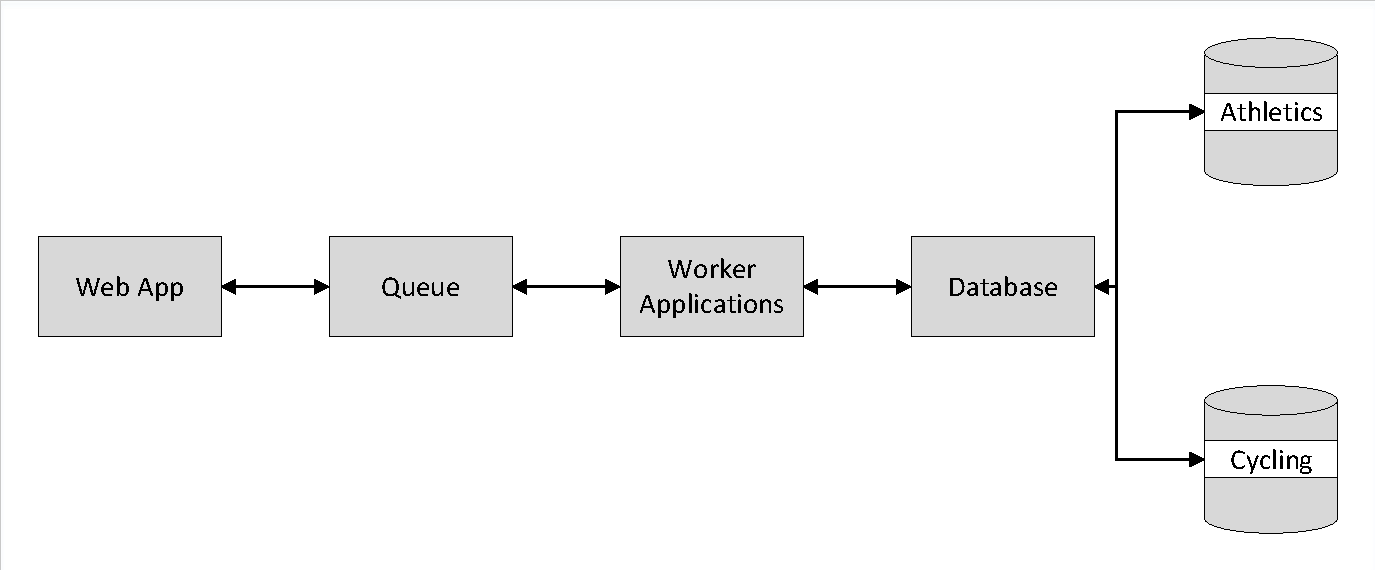
\includegraphics[trim = 5 5 5 5, clip, width=\textwidth]{img/sharedqueue}
	\caption{Shared queue middleware architecture}
	\label{figure:queuedd_architecture}
\end{figure}

\begin{figure}
	\centering
	% Automatically generated by PEPA2Latex
	% --begin
	\begin{displaymath}
	\begin{array}{rcl}
	\mathit{a} & = & 1.0\\
	\mathit{c} & = & 1.0\\
	\mathit{q} & = & 100.0\\
	\mathit{db} & = & 5.0\\
	[2.0ex]		\mathit{Website} & \rmdef & (\mathit{athletics},\mathit{a}).\mathit{Website}+(\mathit{cycling},\mathit{c}).\mathit{Website}\\
	\mathit{Q_0} & \rmdef & (\mathit{athletics},\top).\mathit{Q_A}+(\mathit{cycling},\top).\mathit{Q_C}\\
	\mathit{Q_A} & \rmdef & (\mathit{queueA},\top).\mathit{Q_0}\\
	\mathit{Q_C} & \rmdef & (\mathit{queueC},\top).\mathit{Q_0}\\
	[2.0ex]		\mathit{DB_1} & \rmdef & (\mathit{queueA},\mathit{q}).\mathit{DBsrv_1}\\
	\mathit{DBsrv_1} & \rmdef & (\mathit{dbsrv1},\mathit{db}).\mathit{DB_1}\\
	\mathit{DB_2} & \rmdef & (\mathit{queueC},\mathit{q}).\mathit{DBsrv_2}\\
	\mathit{DBsrv_2} & \rmdef & (\mathit{dbsrv2},\mathit{db}).\mathit{DB_2}\\
	\mathit{Service_1} & \rmdef & (\mathit{dbsrv1},\mathit{db}).\mathit{Service_1}\\
	\mathit{Service_2} & \rmdef & (\mathit{dbsrv2},\mathit{db}).\mathit{Service_2}\\
	[2.0ex]		\multicolumn{3}{l}{\mathit{Website}\sync{\substack{athletics\\cycling}}\mathit{Q_0}[10]\sync{\substack{queueA\\queueC}}\mathit{DB_1}\parallel\mathit{DB_2}\sync{\substack{dbsrv1\\dbsrv2}}\mathit{Service_1}\parallel\mathit{Service_2}}\\
	[2.0ex]	\end{array}
	\end{displaymath}
	% --end
	\caption{Shared queue and distributed database}
	\label{figure:queuedd}
\end{figure}

As is now usual, the Eclipse plugin is used to find the steady-state throughputs of the activities for input rates of athletics requests increasing from 1.0 to 10.0 with cycling and other rates fixed.  The results appear numerically in Table \ref{table:queuedd_results} and as a chart comparing {\itshape athletics} and {\itshape cycling} throughput in Figure \ref{figure:queueddnr_sport}.
They show:
\begin{itemize}
	\item the throughput of {\itshape athletics} is constrained by the database service rate of a single node.  Athletics and cycling activities demonstrate loss of throughput, but less than shown for the distributed database component alone.  This may indicate the effect of the middleware queue.	
	\item the throughput of {\itshape cycling} is constrained by the ratio between the input rates of athletics and cycling, as it was with the shared queue component.  The behaviour of the queue appears to be the most significant when combined into a system.
	\item the database node throughput follows the throughput of each sport activity, i.e. the partitioning strategy routes all the demand onto the node handling that sport.
\end{itemize}

\begin{table}[h!]
	\centering
	\caption{Shared queue and distributed database experimental results}
	\label{table:queuedd_results}
	\pgfplotstabletypeset[
	col sep=comma,
	string type,
	columns/a/.style={column name=a, column type={p{.1\textwidth}}},
	columns/athletics/.style={column name=athletics, column type={p{.1\textwidth}}},
	columns/cycling/.style={column name=cycling, column type={p{.1\textwidth}}},
	columns/ratio/.style={column name=ratio, column type={p{.1\textwidth}}},
	columns/qa/.style={column name=queueA, column type={p{.1\textwidth}}},
	columns/qc/.style={column name=queueC, column type={p{.1\textwidth}}},
	columns/dbsrv1/.style={column name=dbsrv1, column type={p{.1\textwidth}}},
	columns/dbsrv2/.style={column name=dbsrv2, column type={p{.1\textwidth}}},
	every head row/.style={before row=\hline Rate & \multicolumn{7}{c}{Throughput} \\,after row=\hline},
	every last row/.style={after row=\hline},
	]{data/qddnr/results.csv}
\end{table}

\begin{figure}
	\centering
	\begin{tikzpicture}
	\begin{axis}[
	title={Throughput against input rate a},
	width=0.7\textwidth,
	xlabel={Rate a},
	ylabel={Throughput},
	xmin=0, xmax=10,
	ymin=0, ymax=5,
	legend pos=north west,
	ymajorgrids=true,
	grid style=dashed,
	cycle multiindex* list={
		mark list*
		\nextlist
		cyan,brown,green,blue,red
	}
	]
	
	\addplot table [x index={0}, y index={1}, col sep=comma]{data/qddnr/athletics.csv};
	\addplot table [x index={0}, y index={1}, col sep=comma]{data/qddnr/cycling.csv};
	
	\legend{athletics,cycling}
	
	\end{axis}
	\end{tikzpicture}
	\caption{Shared queue and distributed database - sport throughput}
	\label{figure:queueddnr_sport}
\end{figure}

%
% ---- Shared queue and distributed database with replication
%
\FloatBarrier
\subsection{Shared queue and distributed database with replication}

The final system model (Figure \ref{figure:queueddrep_architecture}) combines a shared queue with a distributed database using replication, with one replica of each data partition on the `next' node using consistent hashing.  As before the website sends ticket requests via a shared queue to a worker application, which dequeues them for the database.

The PEPA model (Figure \ref{figure:queueddrep}) combines the shared queue and distributed database with replication components, so that there is now an additional queue state $\mathit{Q_D}$ for holding {\itshape diving} ticket requests, and there are three data node processes.  $\mathit{DB_1}$ is able to service {\itshape athletics} and {\itshape cycling} requests,  $\mathit{DB_2}$ handles {\itshape cycling} and {\itshape diving}, and $\mathit{DB_3}$ handles {\itshape athletics} and {\itshape diving}.  As with the component node, the model's assumption is that each data node handles each supported sport with equal probability.  Again the model uses a queue length of N=10 and maximum queue worker rate of $\mathit{q=100.0}$.

\begin{figure}
	\centering
	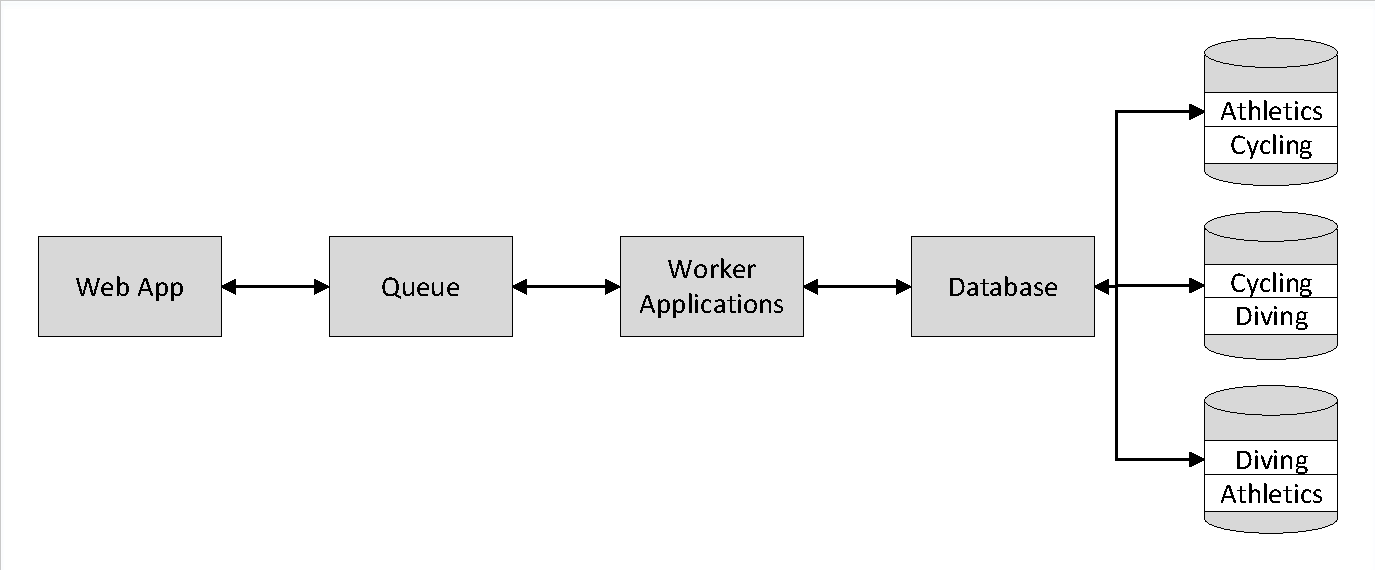
\includegraphics[trim = 5 5 5 5, clip, width=\textwidth]{img/sharedqueue_withrep}
	\caption{Distributed database with replication architecture}
	\label{figure:queueddrep_architecture}
\end{figure}

\begin{figure}
	\centering
	% Automatically generated by PEPA2Latex
	% --begin
	\begin{displaymath}
	\begin{array}{rcl}
	\mathit{a} & = & 1.0\\
	\mathit{c} & = & 1.0\\
	\mathit{d} & = & 1.0\\
	\mathit{q} & = & 100.0\\
	\mathit{db} & = & 5.0\\
	[2.0ex]		\mathit{Website} & \rmdef & (\mathit{athletics},\mathit{a}).\mathit{Website}+(\mathit{cycling},\mathit{c}).\mathit{Website}+(\mathit{diving},\mathit{d}).\mathit{Website}\\
	\mathit{Q_0} & \rmdef & (\mathit{athletics},\top).\mathit{Q_A}+(\mathit{cycling},\top).\mathit{Q_C}+(\mathit{diving},\top).\mathit{Q_D}\\
	\mathit{Q_A} & \rmdef & (\mathit{queueA},\top).\mathit{Q_0}\\
	\mathit{Q_C} & \rmdef & (\mathit{queueC},\top).\mathit{Q_0}\\
	\mathit{Q_D} & \rmdef & (\mathit{queueD},\top).\mathit{Q_0}\\
	[2.0ex]		\mathit{DB_1} & \rmdef & (\mathit{queueA},\mathit{q}).\mathit{DBsrv_1}+(\mathit{queueC},\mathit{q}).\mathit{DBsrv_1}\\
	\mathit{DBsrv_1} & \rmdef & (\mathit{dbsrv1},\top).\mathit{DB_1}\\
	\mathit{DB_2} & \rmdef & (\mathit{queueC},\mathit{q}).\mathit{DBsrv_2}+(\mathit{queueD},\mathit{q}).\mathit{DBsrv_2}\\
	\mathit{DBsrv_2} & \rmdef & (\mathit{dbsrv2},\top).\mathit{DB_2}\\
	\mathit{DB_3} & \rmdef & (\mathit{queueD},\mathit{q}).\mathit{DBsrv_3}+(\mathit{queueA},\mathit{q}).\mathit{DBsrv_3}\\
	\mathit{DBsrv_3} & \rmdef & (\mathit{dbsrv3},\top).\mathit{DB_3}\\
	\mathit{Service_1} & \rmdef & (\mathit{dbsrv1},\mathit{db}).\mathit{Service_1}\\
	\mathit{Service_2} & \rmdef & (\mathit{dbsrv2},\mathit{db}).\mathit{Service_2}\\
	\mathit{Service_3} & \rmdef & (\mathit{dbsrv3},\mathit{db}).\mathit{Service_3}\\
	[2.0ex]		\multicolumn{3}{l}{\mathit{Website}\sync{\substack{athletics\\cycling\\diving}}\mathit{Q_0}[10]\sync{\substack{queueA\\queueC\\queueD}}\mathit{DB_1}\parallel\mathit{DB_2}\parallel\mathit{DB_3}\sync{\substack{dbsrv1\\dbsrv2\\dbsrv3}}\mathit{Service_1}\parallel\mathit{Service_2}\parallel\mathit{Service_3}}\\
	[2.0ex]	\end{array}
	\end{displaymath}
	% --end
	\caption{Shared queue and distributed database with replication}
	\label{figure:queueddrep}
\end{figure}

\FloatBarrier
Experiments are performed in the Eclipse plugin with the usual input rates.  The resulting steady state throughputs are shown in Table \ref{table:queueddwr_results}, in Figure \ref{figure:queueddwr_sport} as a chart comparing {\itshape athletics} and {\itshape cycling} throughput (as the cycling and diving throughputs are identical), and in Figure \ref{figure:queueddwr_database} showing the throughput of the database nodes.
They show:
\begin{itemize}
	\item the throughput of {\itshape athletics} is still constrained but is greater than that of a single database node.  The demand is shared between both data nodes supporting athletics requests.
	\item the throughput of {\itshape cycling} (and diving) is constrained by the ratio between the input rates of athletics and cycling.  In the component model, {\itshape cycling} and {\itshape diving} were impacted by athletics as they both shared a node with athletics tickets.  In the system model, the queue effect appears to outweigh this.
	\item the database node throughput of the two nodes supporting athletics requests is equal, and both are higher than the remaining data node that supports only cycling and diving.  The throughput of this node increases with athletics throughput up to a point, suggesting the node is handling an increasing proportion of the demand for cycling and diving tickets (but that this demand becomes constrained by the queue effect).
\end{itemize}

\begin{table}[h!]
	\centering
	\caption{Shared queue and distributed database with replication experimental results}
	\label{table:queueddwr_results}
	\pgfplotstabletypeset[
	col sep=comma,
	string type,
	columns/a/.style={column name=a, column type={p{.07\textwidth}}},
	columns/athletics/.style={column name=athletics, column type={p{.1\textwidth}}},
	columns/cycling/.style={column name=cycling, column type={p{.1\textwidth}}},
	columns/diving/.style={column name=diving, column type={p{.1\textwidth}}},
	columns/ratio/.style={column name=ratio, column type={p{.07\textwidth}}},
	columns/qa/.style={column name=queueA, column type={p{.09\textwidth}}},
	columns/qc/.style={column name=queueC, column type={p{.09\textwidth}}},
	columns/qd/.style={column name=queueD, column type={p{.09\textwidth}}},
	columns/dbsrv1/.style={column name=dbsrv1, column type={p{.09\textwidth}}},
	columns/dbsrv2/.style={column name=dbsrv2, column type={p{.09\textwidth}}},
	columns/dbsrv3/.style={column name=dbsrv3, column type={p{.09\textwidth}}},
	every head row/.style={before row=\hline Rate & \multicolumn{10}{c}{Throughput} \\,after row=\hline},
	every last row/.style={after row=\hline},
	]{data/qddwr/results.csv}
\end{table}

\begin{figure}
	\centering
	\begin{tikzpicture}
	\begin{axis}[
	title={Throughput against input rate a},
	width=0.7\textwidth,
	xlabel={Rate a},
	ylabel={Throughput},
	xmin=0, xmax=10,
	ymin=0, ymax=9,
	legend pos=north west,
	ymajorgrids=true,
	grid style=dashed,
	cycle multiindex* list={
		mark list*
		\nextlist
		cyan,brown,green,blue,red
	}
	]
	
	\addplot table [x index={0}, y index={1}, col sep=comma]{data/qddwr/athletics.csv};
	\addplot table [x index={0}, y index={1}, col sep=comma]{data/qddwr/cycling.csv};
	
	\legend{athletics,cycling}
	
	\end{axis}
	\end{tikzpicture}
	\caption{Shared queue and distributed database with replication - sport throughput}
	\label{figure:queueddwr_sport}
\end{figure}

\begin{figure}
	\centering
	\begin{tikzpicture}
	\begin{axis}[
	title={Throughput against input rate a},
	width=0.7\textwidth,
	ybar=0pt,
	bar width=.015\textwidth,
	xlabel={Rate a},
	ylabel={Throughput},
	xtick=data,
	ymin=0, ymax=6,
	legend pos=north west,
	ymajorgrids=true,
	grid style=dashed,
	]
	
	\addplot [pattern=north east lines, pattern color=blue] table [x index={0}, y index={1}, col sep=comma]{data/qddwr/dbsrv_1.csv};
	\addplot [fill=green] table [x index={0}, y index={1}, col sep=comma]{data/qddwr/dbsrv_2.csv};
	\addplot [pattern=crosshatch, pattern color=brown] table [x index={0}, y index={1}, col sep=comma]{data/qddwr/dbsrv_3.csv};
	
	\legend{dbsrv1,dbsrv2,dbsrv3}
	
	\end{axis}
	\end{tikzpicture}
	\caption{Shared queue and distributed database with replication - database throughput}
	\label{figure:queueddwr_database}
\end{figure}

%
% ---- System comparison
%
\FloatBarrier
\subsection{Comparison}

As the experiments on the three system models all used the same range of input rates {\itshape a} and {\itshape c}, and the throughput of {\itshape athletics} and {\itshape cycling} requests was recorded for each system, then their experimental results may be compared with each other. (Caveat: only the distributed database with replication model has the additional {\itshape diving} activity, but its throughput was identical to diving).  The {\itshape db} rate of the simple microservices model has been set back to 5.0, the same as the other models, and the numerical results of each system model test are compared in Table \ref{table:comparison_results}.  If the models prove to be good representations of built systems, then such comparison shows the strengths and weaknesses of particular distributed system architectures and provides information for decision-making in their selection during design.

\begin{table}[h!]
	\centering
	\caption{Comparison of system results}
	\label{table:comparison_results}
	\pgfplotstabletypeset[
	col sep=comma,
	string type,
	columns/a/.style={column name=a, column type={p{.1\textwidth}}},
	columns/amicro/.style={column name=athletics, column type={p{.15\textwidth}}},
	columns/cmicro/.style={column name=cycling, column type={p{.15\textwidth}}},
	columns/aqddnr/.style={column name=athletics, column type={p{.15\textwidth}}},
	columns/cqddnr/.style={column name=cycling, column type={p{.15\textwidth}}},
	columns/aqddwr/.style={column name=athletics, column type={p{.15\textwidth}}},
	columns/cqddwr/.style={column name=cycling, column type={p{.15\textwidth}}},
	every head row/.style={before row=\hline Rate & \multicolumn{2}{l}{Simple Microservices} & \multicolumn{2}{l}{Queue + Distributed DB} & \multicolumn{2}{l}{Queue + DB with Replication} \\,after row=\hline},
	every last row/.style={after row=\hline},
	]{data/compare.csv}
\end{table}

\paragraph{Athletics Throughput.}  The comparison shows that the actual throughput of the skewed demand for athletics tickets is lowest for the simple microservices system.  Introducing queue middleware to the system gives a throughput much closer to the maximum service rate of a database node.  Using a distributed database with replication has a load sharing effect so that this system comes closest of all to a throughput that meets the demand.

\paragraph{Cycling Throughput.}  In contrast, the cycling throughput is overall higher for the simple microservices system.  At lower levels of athletics demand, the queue-based systems win out, but as the skewed demand increases then it begins to have an impact on the cycling throughput in these systems.  As the microservices architecture isolates cycling from athletics, it remains at a constant rate.

%
% ---- Built systems
%
\FloatBarrier
\section{Built systems}\label{sec:built-systems}

To test the results predicted by the PEPA system models, actual systems using those architectures are built and their throughputs measured under simulated workloads.

\subsection{Implementation}

\subsubsection{Shared Design.}  All three systems were developed in Java and deployed on Microsoft Azure virtual machines.  The system designs discuss their specifics.  All use a Cassandra database or databases with the same ticket schema design, given in Figure \ref{figure:cassandra_ticket_schema}, with 500 tickets of each sport.

Cassandra was chosen as the distributed database models were designed for consistent hashing (most relevant for the model using replication).  Although the simple microservices model need not have used Cassandra databases, reusing the schema design and database servers was an economical choice, and it illustrates how different architectures may arrange many of the same components.

The source code for the systems and related tools is hosted on GitHub \cite{RN1073}.

\begin{figure}
	\centering
	\begin{lstlisting}[basicstyle=\ttfamily]
	/*
	* int id - unique ticket id
	* varchar sport - type of sport
	* int day - day of event
	* int seat - seat number
	* varchar owner - name of booked ticket owner
	* 
	* The partition key is sport
	* The clustering columns are owner, day, id
	*/
	
	CREATE TABLE IF NOT EXISTS ticket (
	id int,
	sport varchar,
	day int,
	seat int,
	owner varchar,
	PRIMARY KEY (sport, owner, day, id)
	) WITH comment = 'Tickets';
	\end{lstlisting}
	\caption{Cassandra database ticket schema}
	\label{figure:cassandra_ticket_schema}
\end{figure}

\subsubsection{Workload Simulation.}  The workload from a web application and its users was simulated using Apache JMeter \cite{RN1074}, a Java application for load testing.  JMeter was originally designed for testing web applications and all the systems have RESTful APIs over HTTP (for the simple microservices architecture, the Java Spring APIs; for the shared queue architectures, the Microsoft Azure Storage Queue REST APIs).  JMeter test plans are composed of thread groups, where the number of threads and test executions are specified, samplers such as HTTP Request, and timers to determine the delay between each test execution.  Increasing the number of threads used in the test increases the required demand.  JMeter's Poisson Random Timer is used to simulate the negative exponential distribution \cite{RN80} that PEPA steady state solutions assume.

\subsubsection{Measurement.}  Measurement of throughputs in the built systems is required to produce results that can be compared with the PEPA model experimental results.

\paragraph{Measurands.} The measurands are the throughputs of athletics and cycling requests in the worker applications, and control requests that do not access the database in order to show any system overheads.  Where applicable, measurands include the throughputs of diving requests and database queries.

\paragraph{Measurement method.}  The worker applications are measured using Coda Hale Metrics \cite{RN1079}, a Java library providing instrumentation.  The instrument used is a {\itshape Meter}, that measures the rate at which events occur as mean and moving average rates.  Database throughputs are measured by enabling the built-in Cassandra metric ThreadPools.CompletedTasks.request.ReadStage (the total count of completed read queries).  In both cases the metrics are logged every 10 seconds.

\paragraph{Measurement procedure.} The largest 1-minute moving average over a test run is extracted by a Python script.  For the worker applications, the 1-minute average is provided by the Meter instrument.  For Cassandra metric files, the average must be calculated, again using a Python script.  To reduce the impact of any variable performance of virtual machines in the Cloud, each experiment is carried out five times and the mean is taken of the five sets of results.

%
% ---- Simple microservices
%
\FloatBarrier
\subsection{Simple microservices}

\subsubsection{Design.}  The simple microservices architecture from Figure \ref{figure:simplemicro_architecture} was deployed on four Azure Ubuntu virtual machines as shown in Table \ref{table:builtmicro_vmdesign}.  There are two completely separate Cassandra databases, one containing Athletics tickets, one for Cycling tickets.  There are two instances of the {\itshape SimplemicroApplication} worker application, each running on a separate virtual machine and each connecting to one of the databases.

SimplemicroApplication was built using Java Spring \cite{RN1076}, a framework including architectural design pattern modules for Model-View-Controller (used to implement RESTful APIs for the application) and Repository data access (which supports connection to many databases including Cassandra).  The application has two RESTful APIs:

{\textbackslash search}, which takes a sport parameter (Athletics or Cycling), queries the database for all matching tickets, and records metrics.

{\textbackslash control}, which doesn't access the database, but still records metrics.

\begin{table}[h!]
	\centering
	\caption{Simple microservices Azure VMs}
	\label{table:builtmicro_vmdesign}
	\begin{tabular}{l | l | l}
		VM		& Specification		& Application \\
		\hline
		worker1	& DS1 v2 (1 core, 3.5 GB)	& SimplemicroApplication \\
		worker2	& DS1 v2 (1 core, 3.5 GB)	& SimplemicroApplication \\
		db1		& F1s (1 core, 2 GB)	& Cassandra \\
		db2		& F1s (1 core, 2 GB)	& Cassandra \\
	\end{tabular}
\end{table}

\subsubsection{Workload Simulation.}  The application was tested using JMeter with two thread groups running in parallel, Cycling with a constant 10 threads (users) and Athletics ramping up from 10-100 in steps of 10.  Each thread group had a Poisson random timer with a lambda value of 500 milliseconds and a loop count of 500 requests, ensuring several minutes worth of samples and therefore a number of rolling 1-minute averages.  The test plan was used against the {\textbackslash control} APIs for tuning and calibration, showing that the constant demand was approximately 19 requests per second and the skewed demand ranged from 19-190 requests per second (again, approximately, given that the distribution is random). The test plan was then applied to the {\textbackslash search} API with the same parameters.

\subsubsection{Results.}  The results are given numerically in Table \ref{table:builtmicro_results} and shown graphically in Figure \ref{figure:builtmicro_charts} (where the `control' plot is the control throughput from the athletics virtual machine).  The athletics worker throughput using {\textbackslash search} was measured to be limited to 130 queries per second, compared to the control throughput on the same virtual machine i.e. that is the limit imposed by the database.  Using Cassandra's packaged cassandra-stress load testing tool on the database server shows that it is capable of much higher query rate, which suggests that using Java Spring Data adds overheads to the database requests (perhaps, given the use of sessionless RESTful APIs, the main overhead is setting up a connection session to Cassandra each time).  The PEPA database model has already been acknowledged to be an abstraction which does not include such factors, and the scaled rate was fed back into the model's database service rate.

The cycling throughput is more isolated from athletics than the queue-based systems, but there is a slow downward trend as athletics demand increases, not clearly matched by the control throughput.  This may indicate some level of communication between the otherwise separate Cassandra databases on the same subnet, or co-residency effects on the virtual machines.

\begin{table}[h!]
	\centering
	\caption{Simple microservices experimental results}
	\label{table:builtmicro_results}
	\pgfplotstabletypeset[
	col sep=comma,
	string type,
	columns/ausers/.style={column name=users, column type={p{.15\textwidth}}},
	columns/acontrol/.style={column name=control, column type={p{.15\textwidth}}},
	columns/athletics/.style={column name=search, column type={p{.15\textwidth}}},
	columns/cusers/.style={column name=users, column type={p{.15\textwidth}}},
	columns/ccontrol/.style={column name=control, column type={p{.15\textwidth}}},
	columns/cycling/.style={column name=search, column type={p{.15\textwidth}}},
	every head row/.style={before row=\hline \multicolumn{3}{c}{Athletics worker} & \multicolumn{3}{c}{Cycling worker} \\,after row=\hline},
	every last row/.style={after row=\hline},
	]{data/builtmicro/results.csv}
\end{table}

\begin{figure}
	\centering
	\begin{tikzpicture}
	\begin{axis}[
	title={Throughput against athletics demand},
	width=0.7\textwidth,
	xlabel={Athletics demand (users)},
	ylabel={Throughput},
	xmin=0, xmax=100,
	ymin=0, ymax=200,
	legend pos=north west,
	ymajorgrids=true,
	grid style=dashed,
	cycle multiindex* list={
		mark list*
		\nextlist
		cyan,brown,green,blue,red
	}
	]
	
	\addplot table [x index={0}, y index={2}, col sep=comma]{data/builtmicro/results.csv};
	\addplot table [x index={0}, y index={5}, col sep=comma]{data/builtmicro/results.csv};
	\addplot table [x index={0}, y index={1}, col sep=comma]{data/builtmicro/results.csv};
	
	\legend{athletics,cycling,control}
	
	\end{axis}
	\end{tikzpicture}
	\caption{Simple microservices experimental results}
	\label{figure:builtmicro_charts}
\end{figure}

%
% ---- Shared queue middleware
%
\FloatBarrier
\subsection{Shared queue and distributed database}

\subsubsection{Design.}  The shared queue and distributed database architecture from Figure \ref{figure:queuedd_architecture} was deployed on three Azure Ubuntu virtual machines as shown in Table \ref{table:builtddnr_vmdesign}, and using a single Azure Storage Queue instance.  Azure queues provide their own RESTful API access and JMeter was used to populate the queue with Athletics, Cycling or Control ticket requests.

The {\itshape QueueWorker} application was built as a multithreaded application running on a single, multi-core virtual machine.  It dequeues every request (Athletics, Cycling or Control tickets) from the shared Azure Storage Queue.  This asynchronous middleware would be best suited to the `return ticket' operation from the use case, but to ensure that a usable Cassandra metric was available for measuring database throughput, an Athletics or Cycling request was interpreted as a `search ticket` operation.  A database select of all tickets for the matching sport is carried out first and the metric is recorded if the query returns results.  As before the Control request does not access the database but records metrics.  When connecting to the Cassandra database, the QueueWorker application uses a round-robin algorithm to select the coordinator node, to ensure that any additional overheads incurred are shared equally between both nodes.

As populating the queue with JMeter and processing it with the queue worker application are decoupled, it was possible to run QueueWorker on a prepopulated queue to determine its maximum throughput i.e. regardless of the incoming demand.  Using this technique suggested that maximum performance came with QueueWorker running with 16 threads.

The Cassandra database was distributed using a keyspace (`Distributed') with SimpleStrategy, replication\_factor=1 onto two nodes each on one virtual machine.  Cassandra's partitioning places Athletics tickets on one node, and Cycling tickets on the other.  This was validated using nodetool getendpoints, which shows which node hosts records from a given keyspace matching a given partition key e.g. nodetool getendpoints Distributed ticket Athletics.

Note that without the overheads of starting a new Cassandra database session for each request, it was necessary to slow Cassandra down by turning on tracing for 100\% of queries using nodetool settraceprobability 1.0.  Load testing the database alone with cassandra-stress using 16 threads and a query for all athletics tickets suggested a maximum database throughput of 475 operations per second.

\begin{table}[h!]
	\centering
	\caption{Shared queue and distributed DB Azure VMs}
	\label{table:builtddnr_vmdesign}
	\begin{tabular}{l | l | l}
		VM		& Specification			& Application \\
		\hline
		qworkers	& DS3 v2 Promo (4 cores, 14 GB)	& QueueWorker (16 threads) \\
		db1		& F1s (1 core, 2 GB)		& Cassandra \\
		db2		& F1s (1 core, 2 GB)		& Cassandra \\
	\end{tabular}
\end{table}

\subsubsection{Workload Simulation.}  The application was tested using JMeter with two thread groups running in parallel, Cycling with a constant 15 threads and Athletics ramping up from 15-150 in steps of 15.  Each thread group had a Poisson random timer with a lambda value of 100 milliseconds and a loop count of 1500 requests, ensuring enough samples for a number of rolling 1-minute averages.  Again there was a control version of test plan with the same variables, but sending Control ticket requests to the queue rather than Athletics and Cycling tickets.  This produces constant demand of approximately 95 requests per second and skewed demand from 95-950 requests per second.  Scaling these results with the cassandra-stress measurement about to the model input range of 1-10 suggested keeping the {\itshape db} rate at 5.0.

\subsubsection{Results.} 
Table \ref{table:builtddnr_results} shows the numerical results and Figure \ref{figure:builtddnr_charts} shows the plots of athletics, cycling and control throughputs for the same range of athletics demands stated as the number of JMeter threads or users.

The total throughput of {\itshape athletics} and {\itshape cycling} quickly falls behind the control throughput, and examination of the athletics throughput in particular shows that it is constrained by the database performance of a single node.  Note that the constrained throughout is significantly less than the maximum rate shown by cassandra-stress.  Interestingly the maximum total throughput is still less than that value but much closer to it, so the limit shown by cassandra-stress may be based on the whole cluster even though the tickets only appear on one node.

The {\itshape cycling} throughput is constrained in proportion to the athletics {\itshape demand}, not the actual athletics throughput, so that as the athletics throughput is limited but the demand continues to decrease, then the cycling throughput decreases in the ratio of their respective demands (though the ratio is not exact).  The behaviour of the built system matches the prediction of the model.  The model had a very small queue size, and an actual Azure Storage Queue is practically unlimited, so this result was not certain.

Finally the database node throughput follows the throughput of each sport activity.  The partitioning strategy placed the athletics tickets onto {\itshape db2}, as discovered using nodetool getendpoints, and the throughput on this node increases with the skewed athletics demand.

\begin{table}[h!]
	\centering
	\caption{Shared queue and distributed DB experimental results}
	\label{table:builtddnr_results}
	\pgfplotstabletypeset[
	col sep=comma,
	string type,
	columns/ausers/.style={column name=(users), column type={p{.1\textwidth}}},
	columns/arate/.style={column name=athletics, column type={p{.1\textwidth}}},
	columns/crate/.style={column name=cycling, column type={p{.1\textwidth}}},
	columns/total/.style={column name=total, column type={p{.1\textwidth}}},
	columns/conrate/.style={column name=control, column type={p{.1\textwidth}}},
	columns/ratio/.style={column name=ratio, column type={p{.1\textwidth}}},
	columns/db1/.style={column name=db1, column type={p{.1\textwidth}}},
	columns/db2/.style={column name=db2, column type={p{.1\textwidth}}},
	every head row/.style={before row=\hline Rate & \multicolumn{7}{c}{Throughput} \\,after row=\hline},
	every last row/.style={after row=\hline},
	]{data/builtddnr/results_table.csv}
\end{table}

\begin{figure}
	\centering
	\begin{tikzpicture}
	\begin{axis}[
	title={Throughput against athletics demand},
	width=0.7\textwidth,
	xlabel={Athletics demand (users)},
	ylabel={Throughput},
	xmin=0, xmax=150,
	ymin=0, ymax=1000,
	legend pos=north west,
	ymajorgrids=true,
	grid style=dashed,
	cycle multiindex* list={
		mark list*
		\nextlist
		cyan,brown,green,blue,red
	}
	]
	
	\addplot table [x index={0}, y index={1}, col sep=comma]{data/builtddnr/results_table.csv};
	\addplot table [x index={0}, y index={2}, col sep=comma]{data/builtddnr/results_table.csv};
	\addplot table [x index={0}, y index={4}, col sep=comma]{data/builtddnr/results_table.csv};
	
	\legend{athletics,cycling,control}
	
	\end{axis}
	\end{tikzpicture}
	\caption{Shared queue and distributed DB experimental results}
	\label{figure:builtddnr_charts}
\end{figure}

%
% ---- Distributed database with replication
%
\FloatBarrier
\subsection{Shared queue and distributed database with replication}

\subsubsection{Design.}  The shared queue and distributed database with replication architecture from Figure \ref{figure:queueddrep_architecture} was deployed on four Azure Ubuntu virtual machines as shown in Table \ref{table:builtddwr_vmdesign}, again using a single Azure Storage Queue instance.

The {\itshape QueueWorker} application was reused (as well as handling Athletics, Cycling or Control ticket requests, the application handles Diving requests) and run with 16 threads as before.

The Cassandra database was distributed using a keyspace (`Replicated') with SimpleStrategy, replication\_factor=2 onto three nodes each on one virtual machine.  Cassandra's partitioning places Athletics, Cycling and Diving tickets on different nodes with each node also containing replicas of one other ticket type (it was necessary to use ByteOrderedPartitioner to force this).  This is verified using nodetool getendpoints e.g. nodetool getendpoints Distributed ticket Athletics.

\begin{center}
	\begin{tabular}{l | l | l}
		Node	& Primary	& Replica \\
		\hline
		db1		& Athletics	& Cycling \\
		db2		& Cycling	& Diving \\
		db3		& Diving	& Athletics \\
	\end{tabular}
\end{center}

Again, it was necessary to slow Cassandra down by turning on tracing for 100\% of queries.

Load testing the database with cassandra-stress using 16 threads suggested a maximum database throughput of 600 operations per second.  This suggests that replicating tickets on two database nodes increases the possible throughput, but it hasn't doubled the previous performance of 475 ops per second.  The model keeps the {\itshape db} rate of 5.0 based on that 475 ops per second single-node measurement.

\begin{table}[h!]
	\centering
	\caption{Shared queue and distributed DB with replication Azure VMs}
	\label{table:builtddwr_vmdesign}
	\begin{tabular}{l | l | l}
		VM		& Specification			& Application \\
		\hline
		qworkers	& DS3 v2 Promo (4 cores, 14 GB)	& QueueWorker (16 threads) \\
		db1		& F1s (1 core, 2 GB)		& Cassandra \\
		db2		& F1s (1 core, 2 GB)		& Cassandra \\
		db3		& F1s (1 core, 2 GB)		& Cassandra \\
	\end{tabular}
\end{table}

\subsubsection{Workload Simulation.}  The application was tested using JMeter with three thread groups running in parallel, Cycling and Diving with a constant 15 threads and Athletics ramping up from 15-150 in steps of 15.  The parameters were set to the same values as the previous JMeter test plan.

\subsubsection{Results.} 
Table \ref{table:builtddwr_results} shows the numerical results. Figure \ref{figure:builtddwr_sport} shows the plots of athletics, cycling and control throughputs for the same range of athletics demands.  As for the model, diving throughput is not shown on the chart as it closely matches cycling throughput.  Figure \ref{figure:builtddwr_database} shows the database throughputs for all three nodes.

The control throughput begins to taper off as it gets closer to 1000 requests per second.  Azure queues have a limit of up to 2000 messages per second, so simultaneously queueing and dequeuing requests at the same rate suggests a limit of 1000 messages per second.  The total throughput of {\itshape athletics}, {\itshape cycling} and {\itshape diving} still falls behind control throughput, and again the maximum total is very close to the cassandra-stress limit of 600 requests per second.  Both the total and athletics throughputs are significantly higher than for the system without replication, as predicted by the model.

Again the model correctly predicted that the {\itshape cycling} and {\itshape diving} throughputs would be constrained in a ratio to the athletics throughput that matches (or is close to) the ratio between their demands.

However, the database node throughputs are very different to those from the model.  While the {\itshape db1} and {\itshape db3} nodes that host athletics tickets do show higher throughputs than the node which does not, the throughputs were not shared equally between those two nodes.  Neither was the allocation random.  The average of all five sets of tests showed {\itshape db3} taking many more requests.  This, and the cassandra-stress result showing that the athletics query performance did not double when adding a replica to another node, indicates that Cassandra's performance is more complex than the abstract database model.

\begin{table}[h!]
	\centering
	\caption{Shared queue and distributed database with replication experimental results}
	\label{table:builtddwr_results}
	\pgfplotstabletypeset[
	col sep=comma,
	string type,
	columns/ausers/.style={column name=(users), column type={p{.1\textwidth}}},
	columns/arate/.style={column name=athletics, column type={p{.1\textwidth}}},
	columns/crate/.style={column name=cycling, column type={p{.1\textwidth}}},
	columns/drate/.style={column name=diving, column type={p{.1\textwidth}}},
	columns/total/.style={column name=total, column type={p{.1\textwidth}}},
	columns/conrate/.style={column name=control, column type={p{.1\textwidth}}},
	columns/ratio/.style={column name=ratio, column type={p{.1\textwidth}}},
	columns/db1/.style={column name=db1, column type={p{.1\textwidth}}},
	columns/db2/.style={column name=db2, column type={p{.1\textwidth}}},
	columns/db3/.style={column name=db3, column type={p{.1\textwidth}}},
	every head row/.style={before row=\hline Rate & \multicolumn{9}{c}{Throughput} \\,after row=\hline},
	every last row/.style={after row=\hline},
	]{data/builtddwr/results_table.csv}
\end{table}

\begin{figure}
	\centering
	\begin{tikzpicture}
	\begin{axis}[
	title={Throughput against athletics demand},
	width=0.7\textwidth,
	xlabel={Athletics demand (users)},
	ylabel={Throughput},
	xmin=0, xmax=150,
	ymin=0, ymax=1000,
	legend pos=north west,
	ymajorgrids=true,
	grid style=dashed,
	cycle multiindex* list={
		mark list*
		\nextlist
		cyan,brown,green,blue,red
	}
	]
	
	\addplot table [x index={0}, y index={1}, col sep=comma]{data/builtddwr/results_table.csv};
	\addplot table [x index={0}, y index={2}, col sep=comma]{data/builtddwr/results_table.csv};
	\addplot table [x index={0}, y index={5}, col sep=comma]{data/builtddwr/results_table.csv};
	
	\legend{athletics,cycling,control}
	
	\end{axis}
	\end{tikzpicture}
	\caption{Shared queue and distributed database with replication - sport throughput}
	\label{figure:builtddwr_sport}
\end{figure}

\begin{figure}
	\centering
	\begin{tikzpicture}
	\begin{axis}[
	title={Database throughput against athletics users},
	width=0.7\textwidth,
	ybar=0pt,
	bar width=.015\textwidth,
	xlabel={Athletics users},
	ylabel={Throughput},
	xtick=data,
	ymin=0, ymax=350,
	legend pos=north west,
	ymajorgrids=true,
	grid style=dashed,
	]
	
	\addplot [pattern=north east lines, pattern color=blue] table [x index={1}, y index={2}, col sep=comma]{data/builtddwr/average_db1.csv};
	\addplot [fill=green] table [x index={1}, y index={2}, col sep=comma]{data/builtddwr/average_db2.csv};
	\addplot [pattern=crosshatch, pattern color=brown] table [x index={1}, y index={2}, col sep=comma]{data/builtddwr/average_db3.csv};
	
	\legend{db1,db2,db3}
	
	\end{axis}
	\end{tikzpicture}
	\caption{Shared queue and distributed database with replication - database throughput}
	\label{figure:builtddwr_database}
\end{figure}

%
% ---- Conclusions and Future Work
%
\FloatBarrier
\section{Conclusions and Future Work}\label{sec:conclusions}

This paper met its aims and objectives to demonstrate that PEPA may be used to build models of distributed databases and middleware queues.  Experiments can be run on the models in the PEPA Eclipse plugin to produce steady state throughput results, and make predictions of how the real, built systems will behave under conditions of skewed demand.  These component models may be composed into system models which showed some interesting results, discussed below.  There were mixed results from testing the predictions of the system models against the actual behaviour of built systems.

The models were most successful for qualitative prediction.  They correctly predicted:
\begin{itemize}
	\item that the microservices architecture would better isolate skewed demand from the other components.
	\item (less trivially) when a shared queue is used in combination with a distributed database, once the throughput of resources with skewed demand is choked, the throughput of the other resources was choked in proportion to the relative demand between them and the skewed resource.  This even though the model's queue size is much smaller than an actual Cloud service queue.
	\item where throughput would be routed through a distributed database when using a particular partitioning strategy.
	\item when using a distributed database with replication, there would also be throughput at the replica node, and that therefore the overall throughput of the skewed demand resource would be higher than for a distributed database without replication.
\end{itemize}

However, the models were less accurate at quantitative predictions.  Simple microservices was still best at isolating demand but built system results showed that there was some impact on the other resources.  When using replication, the throughput was not spread evenly (or randomly) between database nodes, and this also meant that the system was unable to satisfy as much demand as predicted.  The models were too abstract to describe and predict the behaviour inside the database engine, or the overheads incurred by worker application design choices.  This meant that the maximum apparent database service rates for actual systems were very different for microservices and the shared queue distributed database models, despite both using the same queries against Cassandra on the same virtual machines.  This means that while the models suggested that they could be used to compare different architectures directly, and to make predictions about which would make the best use of the resources available, the real systems did not bear this out.  The models as they stand are not therefore suitable for right-sizing applications.

It is concluded that the models have demonstrated potential for further work in this application area.

\subsection{Improved Models}

The real Cassandra database behaviour was shown to be more complex than described by these simple models.  One area of future work might be to build on the abstract database model to exhibit the true behaviour more closely.  Care must be taken however not to customise the model so much that it is no longer useful for other database implementations.

\subsection{System Experiments}

The existing models may be used for further experimentation to determine how the currently modelled technologies may be reconfigured to produce better system architectures.  Partitioning strategies normally aim to use all a distributed database's nodes equally.  In such a strategy, what is the impact of skewed demand?  Also, the shared queue led to skewed demand having a significant impact on the other resources, and a valuable subject of further study would be how other queueing strategies might isolate that demand while retaining the advantages of asynchronous middleware.  There are several queue models in \cite{RN75} that would provide a good starting point, e.g. priority queues.

\subsection{Unknown Skewed Demand}
This paper did not consider systems where the source of skewed demand was unknown in advance.  There is much interest in this problem, for example handling flash crowds in peer-to-peer file sharing networks \cite{RN230}.
An interesting area of future work might be in executing the models at runtime to use them for adaptive algorithms, e.g. to change the queueing policy on-demand.  If the models were also improved to the point that they made better quantitative predictions, then they might also be used as an elastic scaling policy and compared with the performance of other right-sizing strategies; control theory, machine learning and other model based techniques including statistical.

\subsection{New Models}
It may also be possible to use PEPA to produce models for other distributed technologies.  For example, a more `natural' microservices architecture would partition the system by operation (Book, Search, Return) with a separate database for each, as shown in Figure \ref{figure:microservices}.  In this architecture the databases maintain eventual consistency via an event streaming application e.g. using Kafka.  The model for this component may well be generalised to a model of publish/subscribe message oriented middleware.

%
% ---- Bibliography ----
%

\bibliographystyle{splncs03}
\bibliography{references}

\end{document}